\documentclass[english, a4paper, 12pt]{article}

% \usepackage[breaklinks,colorlinks=true,citecolor=black,linkcolor=black,urlcolor=cyan,filecolor=black]{hyperref}
\usepackage{hyperref}
\usepackage{times}
\usepackage{graphicx,color}
\usepackage{url}
\usepackage[utf8]{inputenc}
\usepackage{verbatim}
\usepackage{longtable}
\usepackage{tabularx}
\usepackage{multicol}
\usepackage{multirow}
\usepackage{booktabs}
\usepackage{latexsym}
\usepackage{amsmath}
\usepackage{amssymb}

\usepackage{adjustbox}
\usepackage{algorithm}
\usepackage{algorithmic}

\usepackage[english]{babel}
\usepackage{blindtext}
% \usepackage[automark]{scrpage2}
% \pagestyle{scrheadings}
% \clearscrheadfoot 
% \chead{\headmark}
% \ifoot{\invnr} 
% \pagestyle{scrheadings}
\usepackage{lscape}
\usepackage{layout}
\usepackage{rotating}
\usepackage{listings}
\usepackage{array}
\usepackage[inkscapeformat=png]{svg}
\usepackage[printonlyused,withpage]{acronym}
\usepackage{enumitem}

\newcommand{\DV}{GPT-4\xspace}
\usepackage{listings}
\lstset{basicstyle=\ttfamily, columns=flexible, breaklines=true, mathescape=true}

\usepackage{tikz}

\global\setlength{\fboxsep}{0pt}
\usepackage{relsize}
\usepackage{alltt}
\usepackage[most]{tcolorbox}
\tcbset{
  aibox/.style={
    width=474.18663pt,
    top=10pt,
    colback=white,
    colframe=black,
    colbacktitle=black,
    enhanced,
    center,
    attach boxed title to top left={yshift=-0.1in,xshift=0.15in},
    boxed title style={boxrule=0pt,colframe=white,},
  }
}
\newtcolorbox{AIbox}[2][]{aibox,title=#2,#1}

\newcolumntype{L}{>{\centering\arraybackslash}m{3cm}}
\usepackage{color, colortbl}
\definecolor{Gray}{gray}{0.9}

\lstset{
  basicstyle=\ttfamily,
  breaklines=true
  }

\usepackage{blindtext}%
\usepackage{etoolbox}%
\usepackage{microtype}
\usepackage{setspace}
% -------------------- Header and Footer --------------------
\pagenumbering{arabic}
\usepackage{geometry}
\geometry{margin=1in}
\usepackage{fancyhdr}
\pagestyle{fancy}
\fancyhf{}
\fancyhead[L]{\leftmark} % Left header: section name
\fancyfoot[C]{\thepage}   % Center footer: page number
\renewcommand{\headrulewidth}{0.4pt} % header rule
\renewcommand{\footrulewidth}{0.4pt} % footer rule
\renewcommand{\sectionmark}[1]{\markboth{\thesection.\ #1}{}}
\usepackage{afterpage}
\newcommand{\setnextpagestyle}[1]{\afterpage{\clearpage\thispagestyle{#1}}}
\newcommand{\nofootrule}{\renewcommand{\footrulewidth}{0pt}}

% -------------------- Page Layout -------------------- 

\setlength{\topmargin}{2cm}
\setlength{\headheight}{15pt}
\setlength{\headsep}{20pt}
\setlength{\topskip}{12pt}
\setlength{\evensidemargin}{0pt}
\setlength{\oddsidemargin}{0pt}
\setlength{\textheight}{240mm}
\setlength{\textwidth}{160mm}
\setlength{\voffset}{-2cm}
\setlength{\parindent}{20pt}
\setlength{\parskip}{6pt}


\patchcmd{\thebibliography}{\chapter*}{\par\let\clearpage\relax\chapter*}{\typeout{success}}{\typeout{failure}}

% -------------------- New Commands --------------------

\newcommand{\saauthor}{Shahriar Yazdipour}
\newcommand{\matrikel}{62366}
\newcommand{\sathema}{A Review on State-of-the-art \\Text-To-SQL Solutions}

\newcommand{\saprof}{Prof. Dr.-Ing. Patrick Mäder}
\newcommand{\saproff}{M. Sc. Martin Hofmann}

% \newcommand{\invnr}{2020-11-01}



% --------------- subsubsubsection -----------------
\newcommand{\subsubsubsection}[1]{\paragraph{#1}\mbox{}\\}
\setcounter{secnumdepth}{4}
\setcounter{tocdepth}{4}

% -------------------- Title --------------------
\usepackage[T1]{fontenc}
\usepackage{titlesec}
% \titleformat{\section}{\clearpage\thispagestyle{plain}\fontsize{28}{22}\selectfont}{\thesection}{1em}{}

\titleformat{\section}[display]
  {\clearpage\thispagestyle{plain}\fontsize{36}{36}\selectfont\bfseries}
  {\bfseries Chapter \thesection}
  {10pt}
  {\Large}

% -------------------- Caption --------------------
\usepackage{caption}
\captionsetup{skip=5pt,font=small} % Adjust the value as desired
% -------------------- Fonts --------------------
% \usepackage{mathpazo}
\usepackage{times}

% -------------------- Document --------------------
\begin{document}

\thispagestyle{empty}
\begin{titlepage}

    \begin{center}
        \includegraphics[height=2cm]{pics/TU_Logo_RGB_04.jpg}
        \vspace{1cm}

        TECHNISCHE UNIVERSITÄT ILMENAU\\
        Fakultät für Informatik und Automatisierung\\
        \vspace{4cm}
        {\large  Master Thesis} \\
        \vspace{1cm}
        % {\Large \textbf \sathema} \\
        % \textls[40]{\Large \textbf{\sathema}}\\
        \begin{spacing}{1}
            \Large \textbf{A Review on State-of-the-art} \\
            \Large \textbf{Text-To-SQL Solutions}
          \end{spacing}
        \vspace{4cm}
        % {presented by} \\
        % \vspace{0.5cm}
        % {\large \saauthor}\\
        % {Matrikel \matrikel}
        % \vspace{2cm}

        % Supervisors: \\
        % \vspace{0.5cm}
        % \saprof \\
        % \saproff
        \vspace{1cm}
        % Ilmenau, \today
        \begin{tabular}{lll}
            \\
            \textbf{Supervisors:}                   & & \saprof \\[0.5ex]
                     & & \saproff \\[0.5ex]
                                                   & & \\[0.5ex]
            \textbf{Submitted by:}                 & & \saauthor \\[0.5ex]
                                                   & & Matriculation Number \matrikel \\[0.5ex]
                                                   & & \mail \\[0.5ex]
                                                   & & \\[0.5ex]
            \textbf{Submission Date:}              & & \submissiondate \\[0.5ex]
        \end{tabular}
    \end{center}

\end{titlepage}


\subsection*{Dedication}

I dedicate this thesis to the brave and heroic Iranian women who have stood up against oppression and fought for their rights and freedoms. These women, often at significant personal risk, have courageously spoken out against the injustices they have faced and have worked tirelessly to bring about positive change in their country.

Their tireless efforts and dedication to the cause of gender equality and social justice have inspired me and countless others worldwide. I am deeply grateful for their unwavering commitment to making the world a better place for all.

This thesis is also dedicated to the memory of those who have lost their lives in the struggle for equality and justice. Their sacrifice will never be forgotten, and their legacy will inspire future generations to fight for a more just and equitable world.
\\
Also, I express my deepest gratitude to my parents, who have always been my biggest supporters and have believed in me throughout my academic journey. Their love, guidance, and encouragement have been invaluable to me.
\\
Finally, I am also grateful to my professor, Prof. Patrick Mäder and also Martin Hofmann, who has been excellent mentor and guide throughout the process of writing this thesis. Their expertise and support have been instrumental in helping me to complete this work.

\newpage
\tableofcontents
\section*{List of Acronyms}
\begin{acronym}
  \acro{LSTM}{Long Short-Term Memory}
  \acro{BERT}{Bidirectional Encoder Representations from Transformers}
  \acro{ATIS}{Air Travel Information System}
  \acro{NLQ}{Natural Language Query}
  \acro{RDB}{Relational Database}
  \acro{NL2SQL}{Natural Language to SQL}
  \acro{NLG}{Natural Language Generation}
  \acro{SEDE}{Stack Exchange Data Explorer}
  \acro{SEOSS}{Software Engineering in Open Source Systems}
  \acro{OOV}{Out-of-Vocabulary}
  \acro{CBOW}{Continuous Bag-of-Words}
  \acro{ELMo}{Embeddings from Language Models}
  \acro{GNN}{Graph Neural Networks}
  \acro{PLM}{Pre-trained Language Models}
  \acro{MLM}{Masked Language Modeling}
  \acro{IR}{Intermediate Representations}
  \acro{AST}{Abstract Syntax Trees}
  \acro{BPE}{Byte Pair Encoding}
  \acro{T5}{Text-To-Text Transfer Transformer}
  \acro{COLA}{Corpus on Linguistic Acceptability}
  \acro{C4}{Colossal Clean Crawled Corpus}
  \acro{PCFG}{Probabilistic Context-Free Grammar}
  \acro{GPT}{Generative Pre-trained Transformers}
  \acro{LLM}{Large Language Model}
\end{acronym}
\section{Introduction}

Data retrieval in databases is typically done using SQL (Structured Query Language). Text-to-SQL machine learning models are a recent development in state-of-the-art research. The technique is an attractive alternative for many natural language problems, including complex queries and extraction tasks. The text is converted into a SQL query that can be executed on the database. This technique can save time and effort for both developers and end-users by enabling them to interact with databases through natural language queries. Machine learning and knowledge-based resources aid in converting text language to SQL.

Text-to-SQL allows the elaboration of structured data with information about the natural language text in several domains, such as healthcare, customer service, and search engines. It can be used by data analysts, data scientists, software engineers, and end users who want to explore and analyze their data without learning SQL. It can be used in a variety of ways:

\begin{itemize}
    \item Data analysts can use it to generate SQL queries for specific business questions, such as "What are the top ten products sold this month?"
    \item Data scientists can use it to generate SQL queries for machine learning experiments, such as "How does the price of these products affect their sales?"
    \item Businesses can use this technique to automate data extraction and improve efficiency.
    \item End-users who want to explore and analyze their data without learning SQL can use it by clicking on a button on any table or chart in a user interface.
\end{itemize}

Although these Text-to-SQL models may provide a partial solution to this complex problem, humans still have challenges to overcome. Even experienced database administrators and developers can need help with the task of dealing with unfamiliar schema when working on database migration projects. This is often due to the fact that they have never seen the schema before and therefore need to learn how to read and interpret it correctly. Furthermore, it can take time to determine how to make the necessary changes in order to migrate the data from one database to another successfully. In spite of these challenges, it is possible to successfully complete a database migration project with the help of a text-to-SQL model, as long as the model is carefully implemented and the proper steps are taken.

This research study will examine the various natural language processing (NLP) technologies that have been utilized in recent years to convert text language into Structured Query Language (SQL). Specifically, it will explore and compare the most commonly used NLP technologies and review their effects on the effectiveness of the conversion process. Moreover, this study will also analyze the representative datasets and evaluation metrics that are utilized in the current solutions for this challenging task. By doing so, it is our hope that this research study will provide valuable insights into how NLP technologies can be effectively and efficiently utilized in the conversion of text language into SQL.

Additionally, we will undertake a comprehensive study of the SEOSS (Software Engineering Dataset for Text-to-SQL and Question Answering Tasks) dataset from our esteemed researchers at the university. We will then evaluate the execution of this dataset using the most advanced Text-to-SQL model currently available. This will enable us to understand the capabilities of the SEOSS dataset better and help us to make informed decisions.

\subsection{Challenges}

Text-to-SQL is an intricate task, given the complexity and diversity of natural language and the structure and regulations of SQL. One of the most challenging aspects is to decipher the intent and significance of the natural language input, as it can be ambiguous or have varied interpretations. This can result in mistakes when building the corresponding SQL query, like selecting the incorrect table or columns or not recognizing the conditions for filtering or sorting the data. Additionally, the natural language input may contain typos or unknown words, which can complicate the mapping process. Moreover, the query generated may not be in the optimal form, as it has to take into account the various data types, operations, and constraints of the underlying database. Therefore, it is crucial to develop models and algorithms that can accurately map natural language to SQL queries.

Another challenge is dealing with the diverse and dynamic nature of databases, as the schema and data may change over time, and there may be variations in naming conventions and conventions across different databases. This can make it difficult for the model to correctly map the natural language input to the appropriate SQL elements, such as table and column names, and to handle variations in the structure of the SQL queries generated. Additionally, many real-world scenarios require integration with external knowledge bases and ontologies, which can be challenging to handle, especially when the external knowledge needs to be completed or consistent. Furthermore, the system must be robust to different types of user input, such as colloquial or informal language or input that needs to be completed or clarified. Additionally, Text-to-SQL systems must be able to handle errors in the input, such as typos, as well as rare edge cases that may not have been encountered during the training process. Finally, Text-to-SQL systems must be robust to the presence of out-of-vocabulary words and rare edge cases, which can be challenging to handle without significant amounts of labeled data, as well as the need to make accurate predictions with limited training data.

\clearpage
\subsection{Thesis Outline}

In this section, we provide an outline of our thesis.

\begin{itemize}
    \item Introduction: This chapter presents the motivation, challenges, and goals of the thesis, setting the stage for the subsequent chapters.
    \item Technical Background: In this chapter, we discuss early and recent approaches to Text-to-SQL tasks. We also introduce essential terminology, concepts, and methods in the field of natural language processing.
    \item Benchmark Dataset: This chapter provides an overview of single-domain and large-scale cross-domain benchmark datasets used for evaluating Text-to-SQL models.
    \item State-of-the-art Text-to-SQL Methods: We review the most recent and advanced methods for Text-to-SQL tasks, discussing various techniques for data augmentation, encoding, and decoding.
    \item Learning Techniques: This chapter covers the fully supervised and weakly supervised learning techniques used in Text-to-SQL models, exploring the advantages and drawbacks of each.
    \item Evaluation Metrics: In this chapter, we present the commonly used evaluation metrics for assessing the performance of Text-to-SQL models and discuss their limitations and benefits.
    \item Experiments: This chapter details the experiments conducted using SEOSS, GPT, and T5 PICARD on various benchmark datasets, as well as the implementation of the proposed EZ-PICARD method for microservices practices.
    \item Conclusion: We summarize the main findings of the thesis and highlight its contributions to the field of natural language processing and Text-to-SQL tasks.
    \item Discussion and Future Directions: This chapter provides a discussion on the implications of the results, identifies limitations, and suggests potential future research directions to advance the state of the art in Text-to-SQL methods.
    \item Appendix: The appendix contains supplementary materials, such as detailed experimental results, model configurations, and additional resources for further reading.
\end{itemize}

\section{Motivation}

Representative datasets for Text-to-SQL include the WikiSQL\cite{zhong_seq2sql_2017} dataset and
the SPIDER\cite{yu_spider_2019} dataset, which contains more complex SQL queries.

The former case consists of Single Table - Multiple Question and the latter case Multiple Table - Multiple Question.
First, We will take a shallow look at older datasets and why they are no longer used in Text-to-SQL studies.
We will take a look at the difference between these datasets, which made a significant difference in the performance of Text-to-SQL systems.

The top language models and techniques utilized for the Text-To-SQL solution will be studied. We will jump into details of the architecture and backbond of these studies. We will evaluate the success of these researches and how they are different from each other.

After these models' performance review and hardware requirements, it is planned to develop a web application with minimum essentials for average users to access their database with their natural language questions without any SQL knowledge. This application will be open source via Github and accessible for enthusiasts to try this technology on their own.

% ? The state-of-the-art should show the reader a broad overview of techniques available and how they are related to one another in a hierarchical way like a mindmap. Describe the methods briefly and explain the weaknesses and strengths of the methods and how you want to use them to solve your problem.

\section{Background and Literature Review}

The text-to-SQL problem, or NL2SQL, is defined as the following: Given a Natural Language Query (NLQ) on a Relational Database (RDB), produce a SQL query equivalent to the NLQ. Several challenges include ambiguity, schema linking, vocabulary gaps, and user errors.

It has been a holy grail for the database community for over 30 years to translate user queries into SQL. During this section, we will provide a very brief overview of the earlier approaches, especially those that database communities have proposed.

% add image of mindmap here
\begin{figure}[htb]
    \centering
    \includegraphics[width=0.6\textwidth]{pics/mindmap.png}
    \caption{Mindmap of the state-of-the-art}
    \label{fig:mindmap}
\end{figure}

\subsection{Early Approaches}

\subsection{Recent Approaches}

\section{Benchmark Dataset}

Datasets play a crucial role in developing and evaluating Text-to-SQL models for semantic parsing of natural language phrases. A variety of benchmark datasets are available, each with unique characteristics and features. Examples of early datasets include ATIS\cite{dahl-etal-1994-expanding}, GeoQuery\cite{10.1007/3-540-44795-4_40}, and Yelp\cite{10.1145/3133887}, which focus on a single topic and database. More recent datasets, such as WikiSQL\cite{zhong_seq2sql_2017} and Spider\cite{yu_spider_2019}, are larger and cover a broader range of domains.

Additionally, new datasets include more advanced queries to assess the generalization capabilities of models. These benchmark datasets provide a standardized testbed for evaluating the performance of Text-to-SQL models and are widely used in the research community. They vary in complexity, size, and annotation, allowing researchers to evaluate models' performance at different levels and under different scenarios. This chapter will review the top benchmark datasets used in the Text-to-SQL Semantic Parsing community and discuss their significance for the research community.

\subsection{Single-Domain}

\subsubsection{ATIS (Air Travel Information System) and GeoQuery}

ATIS (Air Travel Information System)\cite{dahl-etal-1994-expanding} and GeoQuery\cite{10.1007/3-540-44795-4_40} are two datasets that are frequently utilized for semantic parsing, a technique for converting natural language inquiries into a structured meaning representation. The ATIS dataset consists of audio recordings and hand transcripts of individuals using automated travel inquiry systems to search for information regarding flights. It is structured using a relational schema to organize data from the official airline guide, with 25 tables containing information concerning fares, airlines, flights, cities, airports, and ground services.
All questions concerning this dataset can be answered using a single relational query. This makes it an ideal choice for training deep learning models, as it is designed for a specific domain and the queries are relatively straightforward.

Furthermore, the questions in the ATIS dataset are mainly limited to select and project queries. On the other hand, GeoQuery is made up of seven tables from the US geography database and 880 natural languages to SQL pairings. It includes geographic and topographical characteristics such as capitals, populations, and landforms. While both datasets are regularly employed to train deep learning models, GeoQuery is more comprehensive and provides a wider range of queries than ATIS. This includes join and nested queries, as well as grouping and ordering queries, which are absent in the ATIS dataset. As a result, GeoQuery is better equipped to answer more complex queries, making it a better choice for training AI models.

% A relational schema is used to organize data from the official airline guide in the ATIS corpus. There are 25 tables containing information about fares, airlines, flights, cities, airports, and ground services. All questions related to this dataset can be answered using a single relational query. The relational database uses shorter tables for this dataset to answer queries intuitively.

% Here is an example query from the ATIS dataset: Input is in natural language, and the output is in \lambda calculus.

% \begin{figure}[htb]
%     \centering
%     \includegraphics[width=0.8\textwidth]{pics/db/ATIS.png}
%     \caption{Example from ATIS dataset for semantic parsing}
%     \label{fig:ATIS}
% \end{figure}

% \subsubsection{GeoQuery Dataset}

% United States geography is represented in the Geoquery dataset. About 800 facts are expressed in Prolog. State, city, river, and mountain information can be found in the database. Geographic and topographical attributes such as capitals and populations make up the majority of the attributes.

\subsubsection{IMDb Dataset}

The IMDb dataset is a well-known dataset in the machine learning community. It contains 50,000 reviews from IMDb and has a limit of 30 reviews per movie\cite{maas-EtAl:2011:ACL-HLT2011}. It is noteworthy that the dataset is balanced in terms of positive and negative reviews, which are equally represented. When creating the dataset, reviews with a score of 4 out of 10 were considered negative and those with a score of 7 out of 10 were considered positive. Neural reviews were excluded to maintain the quality of the dataset. The dataset is divided into training and testing datasets, each with an equal portion. To ensure fairness and accuracy in the results, the dataset creators have taken special care to keep the training and testing datasets balanced.

\begin{figure}[htb]
    \centering
    \includegraphics[width=0.8\textwidth]{pics/db/IMDb.png}
    \caption{Database Structure of IMDb dataset}
    \label{fig:IMDb}
\end{figure}

% \newpage % to avoid page break

\subsubsection{Advising Dataset}

The Advising dataset\cite{finegan-dollak-etal-2018-improving} was created in order to propose improvements in text2SQL systems. The creators of the dataset compare human-generated and automatically generated questions, citing properties of queries that relate to real-world applications. The dataset consists of questions from university students about courses that lead to particularly complex queries. The data is obtained from a fictional student database which includes student profile information such as recommended courses, grades, and previous courses. Moreover, in order to obtain the data for the dataset, academic advising meetings were conducted where students were asked to formulate questions they would ask if they knew the database. After obtaining the questions, the creators of the dataset compared the query results with those from other datasets such as ATIS, GeoQuery, and Scholar. It is evident that many of the queries in the Advising dataset were the same as those found in the other datasets.

% \begin{figure}[htb]
%     \centering
%     \includegraphics[width=0.5\textwidth]{pics/db/Advising.png}
%     \caption{Example from Advising dataset \cite{vig_comparison_2019}}
%     \label{fig:Advising}
% \end{figure}

\subsubsection{MAS (Microsoft Academic Search)}

MAS, or Microsoft Academic Search\cite{roy2013the}, is a database of academic and social networks and a collection of queries. It has a total of 17 tables in its database, as well as 196 natural languages to SQL pairs. MAS can handle join, grouping, and nested queries but does not support ordering queries.

There are a few limitations to be aware of when using natural language queries within MAS. Firstly, all-natural language questions must begin with the phrase ”return me” and can not include an interrogative statement or a collection of keywords. Additionally, all queries must follow the proper grammatical conventions.

\clearpage

\subsection{Large Scale Cross-Domain}

\subsubsection{WikiSQL}

WikiSQL\cite{DBLP:journals/corr/abs-1902-01069} consists of 80,654 natural language questions and corresponding SQL queries on 24,241 tables extracted from Wikipedia. Neither the train nor development sets contain the database in the test set. Databases and SQL queries have simplified the dataset's creators' assumptions. This dataset consists only of SQL labels covering a single SELECT column and aggregation and WHERE conditions. Furthermore, all the databases contain only one table.

The datasets in the test set are not present in the train or development sets in the WikiSQL problem definition. Further, the task needs to accept input from several table schemas. The model must therefore be generalized to new databases. However, they used oversimplified assumptions about the SQL queries and databases in order to generate questions and SQL pairings for 24241 databases. They provide WHERE conditions, a single SELECT column, and aggregation in their SQL labels. Additionally, each database only has one table, with no mention of JOIN, GROUP BY, or ORDER BY.

Prior to the release of SPIDER, this dataset was considered to be a benchmark dataset. Using WikiSQL has been the subject of a great deal of research. WikiSQL's "WHERE" clause has been recognized as one of the most challenging clauses to parse semantically, and SQLNet and SyntaxSQL were previous state-of-the-art models.


\begin{figure}[H]
    \centering
    \includegraphics[width=0.5\textwidth]{pics/db/WikiSQL.png}
    \caption{Example from WikiSQL dataset\cite{DBLP:journals/corr/abs-1902-01069}}
    \label{fig:WikiSQL}
\end{figure}

One example of a state-of-the-art Text-to-SQL solution in the WikiSQL benchmark is the Seq2SQL model, which uses a sequence-to-sequence learning framework to map natural language input to SQL queries. The model uses an attention mechanism to align the input and output sequences and a pointer network to handle SQL queries with complex structural dependencies. We will discuss this model in more detail in the next section.
\clearpage
\subsubsection{SPIDER}

% add image spider3.png
\begin{figure}[htb]
    \centering
    \includegraphics[width=0.9\textwidth]{pics/db/Spider3.png}
    \caption{A difficult text-to-SQL task from the Spider dataset.\cite{wang_rat-sql_2021}}
    \label{fig:Spider3}
\end{figure}

The SPIDER database contains 10K questions and 5K+ complex SQL queries covering 138 different domains across 200 databases. As opposed to previous datasets (most of which used only one database), this one incorporates multiple datasets. Creating this dataset took 11 Yale University students, 1,000 man-hours in total.

Spider contains queries with a lot of intricate SQL elements. In comparison to the sum of the previous Text-to-SQL datasets, Spider comprises around twice as many nested queries and ten times as many ORDER BY (LIMIT) and GROUP BY (HAVING) components.

Creating this corpus was primarily motivated by the desire to tackle complex queries and generalize across databases without requiring multiple interactions.

\begin{figure}[htb]
    \centering
    \includegraphics[width=0.6\textwidth]{pics/db/Spider.png}
    \caption{Process of creating SPIDER dataset\cite{yu_spider_2019}}
    \label{fig:Spider}
\end{figure}

Creating a dataset involves three main aspects: SQL pattern coverage, SQL consistency, and question clarity. Several databases from WikiSQL are included in the dataset. The table is complex as it links several tables with foreign keys. In SPIDER, SQL queries include: SELECT with multiple columns and aggregations, WHERE, GROUP BY, HAVING, ORDER BY, LIMIT, JOIN, INTERSECT, EXCEPT, UNION, NOT IN, OR, AND, EXISTS, LIKE.

The complexity of the dataset increases and the accuracy of solutions drops as the number of foreign keys in the database increases. This is mainly due to the difficulty in selecting the relevant column and table names from a complex database schema. Furthermore, complex database schemas present a major challenge for the model to accurately capture the relationship between different tables which involve foreign keys. SQL queries with a higher number of foreign keys tend to join more tables, suggesting a need for more effective methods to encode the connection between tables with foreign keys.

\subsubsection*{SQL Hardness Criteria}

In order to gain a better understanding of how the model performs on different queries, we have divided SQL queries into four difficulty levels: easy, medium, hard, and extra hard. This classification is based on the number of SQL components, selections, and conditions. Queries that contain multiple SQL keywords (e.g., GROUP BY, ORDER BY, INTERSECT, nested subqueries, column selections, aggregators) are generally considered more complex. For example, a query is considered hard if it includes more than two SELECT columns, more than two WHERE conditions, and GROUP BY two columns, or contains EXCEPT or nested queries. If it contains even more additions on top of that, it is considered extra hard.

\begin{figure}[htb]
    \centering
    \includegraphics[width=0.8\textwidth]{pics/db/Spider2.png}
    \caption{Example of Question-Query set from SPIDER\cite{yu_spider_2019}}
    \label{fig:Spider2}
\end{figure}


SPIDER's exact matching accuracy\ref{eval} was 12.4\% compared to existing state-of-the-art models. As a result of its low accuracy, SPIDER presents a strong research challenge. Current SPIDER accuracy is above 75.5\% with an exact set match without values (refers to values in the WHERE clause) and above 72.6\% with values using PICARD\ref{picard}.

The SPIDER challenge is a research competition dedicated to developing cutting-edge Text-to-SQL and Semantic Parsing solutions. In this challenge, participants strive to develop algorithms that can automatically generate structured SQL queries from natural language input, to improve the performance and accuracy of Text-to-SQL models.

In this challenge, numerous state-of-the-art Text-to-SQL solutions have been proposed, such as the Spider model. This model uses a combination of recurrent and convolutional neural networks to learn the mapping between natural language and SQL queries. This model also has a hierarchical structure, which allows it to process the natural language input more effectively, thereby allowing it to handle complex queries and variations in language with greater precision and accuracy. This model successfully generates accurate and efficient SQL queries from natural language inputs.

One difference between the SPIDER and WikiSQL challenges is the specific dataset that is used for evaluation. The SPIDER challenge uses a dataset of complex SQL queries and natural language questions derived from real-world databases, while the WikiSQL challenge uses a dataset of more straightforward SQL queries and natural language questions derived from Wikipedia articles. This difference in the dataset can affect the performance and accuracy of the models on the different tasks.

Another difference is in the evaluation metrics used. The SPIDER challenge evaluates the models using execution accuracy and natural language understanding metrics, while the WikiSQL challenge evaluates the models using only execution accuracy. This difference in the evaluation metrics can affect how the models are trained and their performance on the tasks. We will discuss the evaluation metrics used in the SPIDER challenge in more detail in the next section\ref{eval}.
\subsubsection{SEDE}

\ac{SEDE} \cite{DBLP:journals/corr/abs-2106-05006} is from a popular online question-and-answer platform with more than 3 million questions, and it recently released a benchmark dataset of SQL queries containing 29 tables and 211 columns. This dataset comprises real-world questions from the Stack Exchange website, such as published posts, comments, votes, tags, and awards.

Although these datasets contain a variety of real-world challenges, they still need to be more tricky to parse semantically due to the complexity of the questions they contain. After further analysis of the 12,023 questions asked on the platform, a total of 1,714 have been verified by humans, which makes it an ideal choice for training and validating the model. This benchmark dataset is highly valuable and helpful for research in natural language processing, as it provides an extensive list of real-world challenges that have rarely been seen in other semantic parsing datasets.

\begin{figure}[H]
    \label{fig:sede_sql}
    \begin{AIbox}{An example of a Complex SEDE utterance}
        \vspace{-5px}
        \parbox{1\textwidth}{\scriptsize
        \begin{alltt} 
            {\bf Utterance:} \\ 
            Check if Votes.CreationDate is always a date
            \\
            {\bf Query:} \\
            SELECT Name, Count(*)as [Count], DatePart(Hour, Votes.CreationDate)as [hour],DatePart(Minute, Votes.CreationDate)as [minute],DatePart(Second, Votes.CreationDate)as [second],DatePart(Millisecond, Votes.CreationDate)as [ms] FROM Votes JOIN VoteTypes ON VoteTypeId = VoteTypes.Id GROUP BY Name, DatePart(Hour, Votes.CreationDate),DatePart(Minute, Votes.CreationDate),DatePart(Second, Votes.CreationDate),DatePart(Millisecond, Votes.CreationDate)
        \end{alltt}
        }
        \vspace{-5px}
    \end{AIbox}
    
    \captionsetup{font={scriptsize,color=white}, skip=-20pt}
    \caption{An example of a Complex SEDE utterance}
\end{figure}
\subsubsection{SEOSS}
% TODO: need more rephrasing

SEOSS dataset is a compilation of natural language expressions with seven alternative phrasings, each linked to a single SQL query. In total, 166 questions (expressions) were organized. The natural language expressions were mainly obtained from existing literature and modified to match the data identified in the issue tracking system (ITS) and version control system (VCS) of an existing software project (namely Apache Pig). This data was extracted and saved into an SQLite database by Rath et al. \cite{RATH2019104005}.

Expressions are labeled into two different tags, development and research. Eighty-one queries with a focus on software needs of stakeholders and developers or from typical use cases' queries of issue tracking systems were labeled as 'development,' and 63 queries containing issue tracking systems information or version control systems were labeled as 'research.' Also, 22 records were generated from the content in questions stakeholders asked within the comment sections of issues of type bug, enhancement/improvement, new feature/feature request, and tasks of 33 open-source Apache projects, which were extracted and stored into databases by Rath and Mäder\cite{RATH2019104005}.

% add image
\begin{figure}[htb]
    \centering
    \includegraphics[width=0.8\textwidth]{pics/seoss/pig.png}
    \caption{Database Schema of the PIG Database \cite{TOMOVA2022108211}}
    \label{fig:SESS}
\end{figure}

% TODO: need more about the Hardness of the SEOSS dataset
% \begin{figure}[htb]
%     \centering
%     \includegraphics[width=0.8\textwidth]{pics/seoss/seoss.png}
%     \caption{Examples of queries with different levels of complexity in SEOSS-Queries Dataset \cite{TOMOVA2022108211}}
%     \label{fig:SESS2}
% \end{figure}

In SEOSS-Queries\cite{TOMOVA2022108211} research, they experienced RatSQL and SQLNet methods on the SEOSS dataset and released their evaluation steps. In this research, we will use the same dataset to evaluate state-of-the-art models currently available in the literature and used in SPIDER for this dataset.

\clearpage


In this chapter, we have reviewed various datasets widely used in the Text-to-SQL Semantic Parsing community. These datasets vary in complexity, size, and annotation, providing a standardized testbed for evaluating the performance of Text-to-SQL models. We have discussed their unique characteristics and features from early datasets such as ATIS and GeoQuery to more recent datasets such as WikiSQL and Spider.
The datasets discussed in this chapter are a valuable resource for the research community to evaluate the progress and performance of Text-to-SQL models. The continued development and improvement of these datasets will be necessary for advancing the field of Text-to-SQL Semantic Parsing.
The table\ref{tab:datasets} below provides an overview of the datasets mentioned in this chapter, including the number of queries and questions sorted by year.

\begin{table}[!ht]
    \centering
    \begin{tabular}{|c|c|c|c|c|c|}
        \hline
        \textbf{Dataset} & \textbf{Year} & \textbf{Tables} & \textbf{Questions} & \textbf{Unique Queries} & \textbf{Domain}            \\ \hline
        ATIS
                         & 1994          & 25              & 5280               & 947                     & Air Travel Information     \\ \hline
        GeoQuery
                         & 2001          & 8               & 877                & 246                     & US geography database      \\ \hline
        Academic
                         & 2014          & 15              & 196                & 185                     & Microsoft Academic Search  \\ \hline
        IMDB
                         & 2015          & 16              & 131                & 89                      & Internet Movie Database    \\ \hline
        Scholar
                         & 2017          & 7               & 817                & 193                     & Academic Publications      \\ \hline
        Yelp
                         & 2017          & 7               & 128                & 110                     & Yelp Movie Website         \\ \hline
        WikiSQL
                         & 2017          & 24,241          & 80,654             & 77,840                  & Wikipedia                  \\ \hline
        Advising
                         & 2018          & 10              & 4570               & 211                     & Student Course Information \\ \hline
        Spider
                         & 2018          & 645             & 10,181             & 5693                    & 138 Different Domains      \\ \hline
        SEDE
                         & 2021          & 29              & 12,023             & 11,767                  & Stack Exchange             \\ \hline
        SEOSS
                         & 2022          & 13              & 1,162              & 116                     & Project ITS and VSC        \\ \hline
    \end{tabular}
    \caption{Comparison of datasets (Sort by Year)}
    \label{tab:datasets}
\end{table}

\section{State-of-the-art Text-To-SQL Methods}

\begin{figure}[htb]
  \centering
  \includegraphics[width=1\textwidth]{pics/Timeline.png}
  \caption{\small Text-to-SQL over time}
  \label{fig:timeline}
\end{figure}

This section will discuss existing cross-domain state-of-the-art (SOTA), text-to-SQL models, beginning with a broad overview and moving on to individual modules. This will provide a clear picture of the progress made in text-to-SQL research. Experiments have shown that pre-trained embeddings improve models because they construct better schema linking and a more accurate SQL structure.

An efficient text-to-SQL solution requires state-of-the-art natural language processing techniques.
As a result of the neural network's capacity to take only numerical inputs and not plain text, word embedding has been used to represent numerical words.
Aside from that, in the past few years, language models have evolved to become increasingly popular as a solution for increasing performance in natural language processing tasks.
Believing that words have numerical representations that differ from others, word embeddings aim to map each word to a multidimensional vector, incorporating valuable details about the word. In addition to the brute-force creation of one-hot embeddings, researchers have developed highly efficient methods for creating representations that convey a word's meaning and relationships with other words. In most, if not all, Text-to-SQL systems, word embedding techniques such as Word2Vec\cite{DBLP:journals/corr/Rong14}, and WordPiece embeddings\cite{DBLP:journals/corr/WuSCLNMKCGMKSJL16} are used.

Recently Language models have been shown to excel at NL tasks as a new type of pre-trained neural network. It is essential to note that language models are not a substitute for word embeddings since they are neural networks and need a way to transform words into vectors.
Relying on the specific problem they want to solve, researchers can adapt the pre-trained model's inputs and outputs and train it for an additional number of epochs on their dataset. Thus, we can achieve state-of-the-art performance without complex architectures \cite{DBLP:journals/corr/abs-1810-04805}. Recent neural network architectures, like the Transformer\cite{https://doi.org/10.48550/arxiv.1706.03762}, have been used to achieve such performance by these models, which excel at handling NL and sequences of NL that are characterized by connections between words. Several language models have been used to handle the text-to-SQL task, including BERT \cite{DBLP:journals/corr/abs-1810-04805}. BERT is a pre-trained language model that has been shown to achieve state-of-the-art performance in various NLP tasks. BERT is a Transformer-based model that utilizes a bidirectional encoder to understand the representation of a word based on the context in which it appears. BERT has been used in several text-to-SQL models, such as BRIDGE \cite{lin_bridging_2020} and RAT-SQL \cite{wang_rat_sql_2021}.



% % add image
% \begin{sidewaysfigure}
%     \centering
%     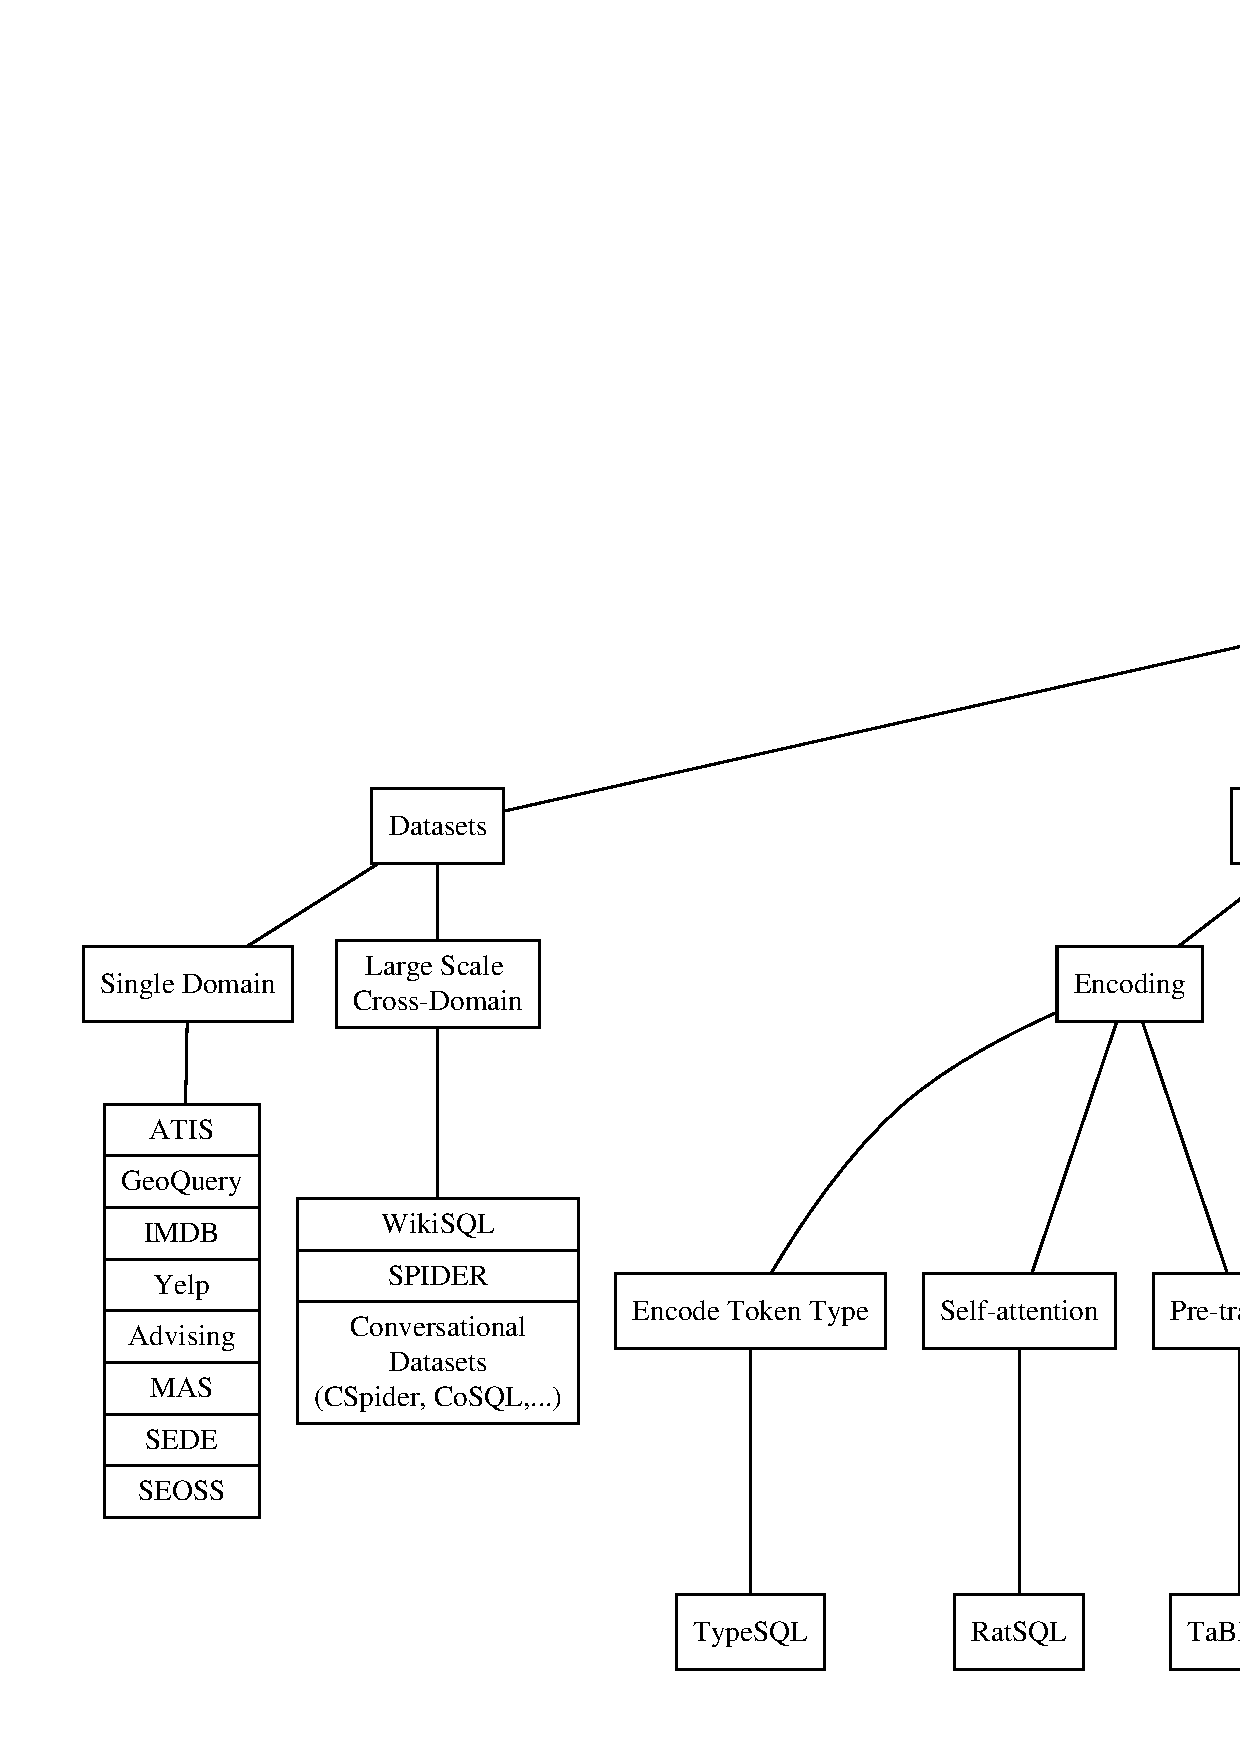
\includegraphics[width=1\linewidth]{pics/mindmap/mind}
%     \caption{Text-to-SQL state-of-the-art Topology}
%     \label{fig:mindmap}
% \end{sidewaysfigure}

\begin{figure}
    \centering
    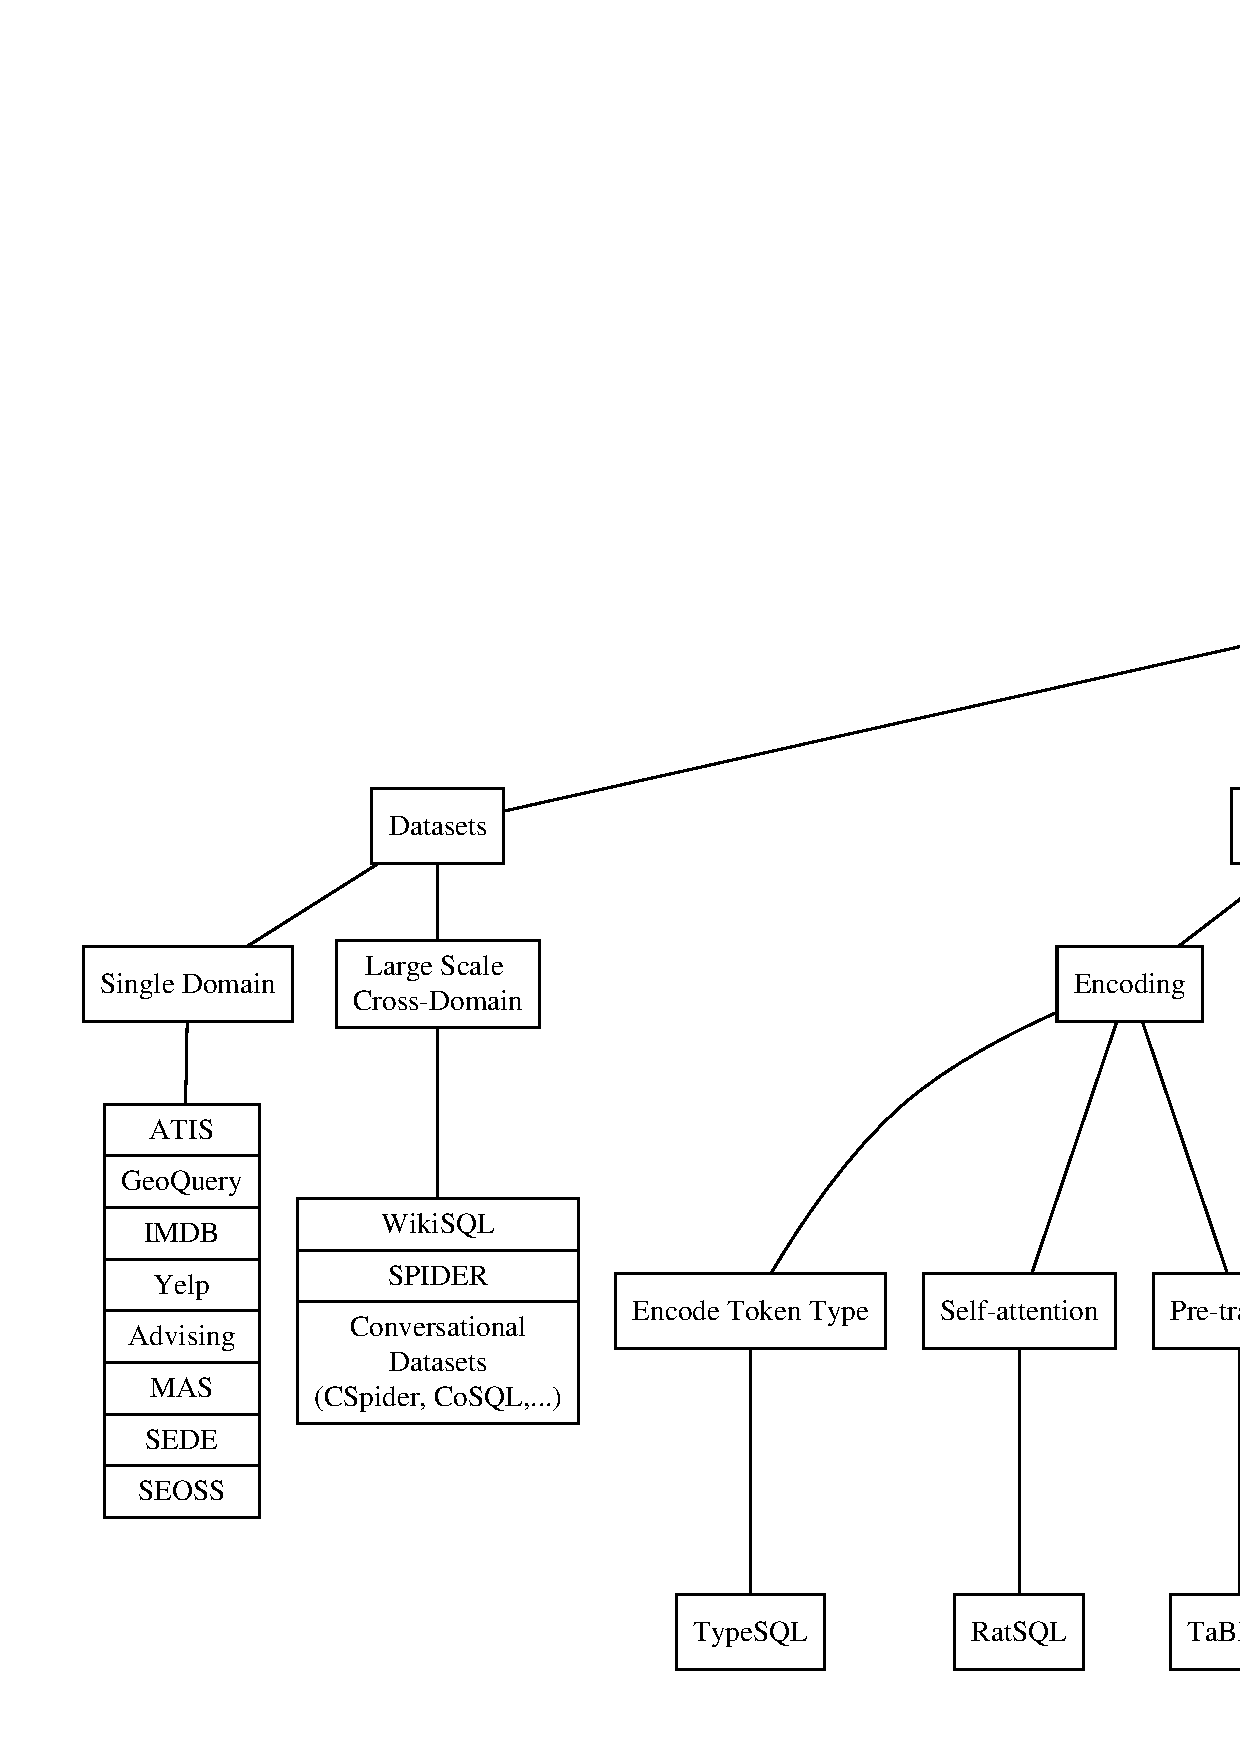
\includegraphics[width=1\linewidth]{pics/mindmap/mind}
    \caption{Text-to-SQL state-of-the-art Topology}
    \label{fig:mindmap}
\end{figure}
\clearpage
\subsection{Encoders}
\label{sec:encoders}

Several approaches have been explored to address the challenges of representing the meaning of questions, capturing the structure of database schemas, and establishing connections between database content and questions in the text-to-SQL domain. These methods play a crucial role in facilitating the understanding of the complex relationships between natural language questions and their corresponding SQL queries.

One of the main challenges in text-to-SQL research is effectively representing the meaning of questions. Various encoding methods have been used to capture the semantics of natural language questions, ranging from traditional word embeddings like Word2Vec and GloVe to more advanced contextualized representations like BERT and its variants. These encoding techniques aim to produce meaningful vector representations of questions that models can use to understand and generate accurate SQL queries.

Another important aspect is representing database schemas, which serve as blueprints for organizing and structuring databases. Researchers have used various strategies to encapsulate database schema information, such as graph-based, tree-structured, and sequence-based encodings. These approaches enable text-to-SQL models to understand the hierarchical relationships and dependencies among various database elements. This allows for more accurate and efficient query generation.

Linking database content to questions is a vital task for text-to-SQL systems. It involves the identification and mapping of relevant entities and attributes from the question to the database schema. To achieve this, various methods have been employed, including attention mechanisms, entity-linking techniques, and schema-agnostic encodings. These approaches help models identify relevant portions of the database schema and generate SQL queries that accurately reflect the intended meaning of the natural language questions.

Encoding methods and encoders play a crucial role in addressing the challenges of representing question semantics, encapsulating database schema structures, and linking database content to questions in the text-to-SQL domain. The exploration of diverse encoding techniques has led to significant advancements in the development of more accurate and efficient text-to-SQL models, furthering the field's understanding of the complex relationships between natural language questions and SQL queries.

\begin{table}
    \centering
    \newcolumntype{g}{>{\columncolor{Gray}}c}
    \begin{tabular}{|c|c|c|c|}
        \hline
        \rowcolor{Gray}
        \textbf{Methods}                & \textbf{Adopted by} & \textbf{Applied datasets} & \textbf{Addressed challenges}                                                                              \\
        \hline

        Encode token type               & TypeSQL             & WikiSQL                   & Representing question meaning                                                                              \\
        \hline
        \multirow{8}{*}{Graph-based}    & GNN                 & Spider                    & \multirow{8}{*}{\parbox{5cm}{Representing question and DB schemas in a structured way and Schema linking}} \\
                                        & Global-GCN          & Spider                    &                                                                                                            \\
                                        & IGSQL               & Sparc, CoSQL              &                                                                                                            \\
                                        & RAT-SQL             & Spider                    &                                                                                                            \\
                                        & LEGSQL              & Spider                    &                                                                                                            \\
                                        & SADGA               & Spider                    &                                                                                                            \\
                                        & ShawdowGNN          & Spider                    &                                                                                                            \\
                                        & S2SQL               & Spider                    &                                                                                                            \\
        \hline
        \multirow{5}{*}{Self-attention} & X-SQL               & WikiSQL                   & \multirow{5}{*}{\parbox{5cm}{Representing question and DB schemas in a structured way and Schema linking}} \\
                                        & SQLova              & WikiSQL                   &                                                                                                            \\
                                        & RAT-SQL             & Spider                    &                                                                                                            \\
                                        & DuoRAT              & Spider                    &                                                                                                            \\
                                        & UnifiedSKG          & WikiSQL, Spider           &                                                                                                            \\
        \hline
        \multirow{4}{*}{Adapt PLM}      & X-SQL               & WikiSQL                   & \multirow{4}{*}{\parbox{5cm}{Leveraging external data to represent question and DB schemas}}               \\
                                        & SQLova              & WikiSQL                   &                                                                                                            \\
                                        & Content Enhanced    & WikiSQL                   &                                                                                                            \\
                                        & HydraNet            & WikiSQL                   &                                                                                                            \\
        \hline
        \multirow{3}{*}{Pre-training}   & TaBERT              & Spider                    & \multirow{3}{*}{\parbox{5cm}{Leveraging external data to represent question and DB schemas}}               \\
                                        & GraPPA              & Spider                    &                                                                                                            \\
                                        & GAP                 & Spider                    &                                                                                                            \\
        \hline
    \end{tabular}
    \caption{Methods used for encoding in text-to-SQL.}
    \label{tab:methods}
\end{table}

\subsubsection{Encode Token Types}

\subsubsection{Graph-based Methods}

\subsubsection{Self-attention}

\subsubsection{Adapt PLM} %Pre-trained Language Models

\subsubsection{Pre-training}

\subsubsection{Ranking-enhanced Encoder}


\clearpage
\section{Decoders}

\begin{table}
    \centering
    \begin{tabular}{|c|c|c|c|}
        \hline
        \rowcolor{Gray}
        \textbf{Methods}                                           & \textbf{Adopted by} & \textbf{Applied datasets} & \textbf{Addressed challenges}                                                            \\
        \hline
        \multirow{3}{*}{Tree-based}                                & Seq2Tree            & -                         & \multirow{3}{*}{Hierarchical decoding}                                                   \\
                                                                   & Seq2AST             & -                         &                                                                                          \\
                                                                   & SyntaxSQLNet        & Spider                    &                                                                                          \\
        \hline
        \multirow{4}{*}{Sketch-based}                              & SQLNet              & WikiSQL                   & \multirow{4}{*}{Hierarchical decoding}                                                   \\
                                                                   &                     & WikiSQL                   &                                                                                          \\
                                                                   & IRNet               & Spider                    &                                                                                          \\
                                                                   & RYANSQL             & Spider                    &                                                                                          \\
        \hline
        Bottom-up                                                  & SmBop               & Spider                    & Hierarchical decoding                                                                    \\
        \hline
        \multirow{2}{*}{Self-Attention}                            & Seq2Tree            & -                         & \multirow{2}{*}{ Synthesizing information}                                               \\
                                                                   & Seq2SQL             & WikiSQL                   &                                                                                          \\
        \hline
        Bi-attention                                               & SmBop               & Spider                    & Synthesizing information                                                                 \\
        \hline
        Structured attention                                       & SmBop               & Spider                    & Synthesizing information                                                                 \\
        \hline
        \parbox{3cm}{Relation-aware Self-attention}                & SmBop               & Spider                    & Synthesizing information                                                                 \\
        \hline
        \multirow{4}{*}{Copy Mechanism}                            & Seq2AST             & -                         & \multirow{4}{*}{ Synthesizing information}                                               \\
                                                                   & Seq2SQL             & WikiSQL                   &                                                                                          \\
                                                                   &                     & WikiSQL                   &                                                                                          \\
                                                                   & SeqGenSQL           & WikiSQL                   &                                                                                          \\
        \hline
        \multirow{6}{*}{\parbox{3cm}{Intermediate Representation}} & IncSQL              & WikiSQL                   & \multirow{6}{*}{{\parbox{5cm}{Bridging the gap between natural language and SQL query}}} \\
                                                                   & IRNet               & WikiSQL                   &                                                                                          \\
                                                                   & ?                   & Spider                    &                                                                                          \\
                                                                   & ?                   & Spider                    &                                                                                          \\  & ?                   & GeoQuery, ATIS
                                                                   &                                                                                                                                            \\  & ?                   & Spider                    &                                                        \\
        \hline
        \multirow{2}{*}{Constrained decoding}                      & UniSAr              & WikiSQL, Spider           & \multirow{2}{*}{Fine-grained decoding}                                                   \\
                                                                   & PICARD              & Spider, CoSQL
                                                                   &                                                                                                                                            \\
        \hline
        \multirow{2}{*}{Execution-guided}                          & SQLova              & WikiSQL                   & \multirow{2}{*}{Fine-grained decoding}                                                   \\
                                                                   & ?                   & WikiSQL
                                                                   &                                                                                                                                            \\
        \hline
        \multirow{2}{*}{Discriminative re-ranking}                 & Global-GCN          &                           & \multirow{2}{*}{SQL Ranking
        }                                                                                                                                                                                                       \\
                                                                   & ?                   & Spider
                                                                   &                                                                                                                                            \\
        \hline
        \multirow{3}{*}{Constrained decoding}                      & SQLNet              & WikiSQL                   & \multirow{3}{*}{Easier decoding
        }                                                                                                                                                                                                       \\
                                                                   & ?                   & WikiSQL
                                                                   &                                                                                                                                            \\
                                                                   & ?                   & Spider
                                                                   &                                                                                                                                            \\
        \hline
        BPE                                                        & UniSAr              & WikiSQL, Spider           & Easier decoding
        \\
        \hline
        Link gating                                                & SmBop               & Spider                    & Synthesizing information                                                                 \\
        \hline
    \end{tabular}
    \caption{Methods used for encoding in text-to-SQL.}
    \label{tab:methods}
\end{table}

\subsection{Tree-based}

\subsection{Sketch-based}

\subsection{Bottom-up}

\subsection{Attention Mechanism}

\subsection{Copy Mechanism}

\subsection{Intermediate Representations}

\subsection{Prevent Invalid Tokens}

\subsection{Skeleton-aware Decoder}

Schema linking is a component of text-to-SQL models that helps map natural language phrases to elements of a database schema.
Skeleton parsing is a component of text-to-SQL models that helps generate the structure of an SQL query based on a natural language question. It focuses on generating the pure skeleton of an SQL query (i.e., SQL keywords).
\clearpage
\subsection{Data Augmentation}
\label{sec:augmentation}

Data augmentation has proven to be an effective technique for improving the performance of text-to-SQL models, allowing them to address more complex or novel questions (Zhong et al. \cite{zhong_semantic_2020} and Wang et al. \cite{wang_rat_sql_2021}), achieve cutting-edge results with less supervised data, and enhance their adaptability to various question types (Radhakrishnan et al. \cite{DBLP:journals/corr/abs-2010-09927}).

Typical data augmentation approaches involve rephrasing questions and employing pre-established templates to boost data variety. Iyer et al. \cite{iyer-etal-2017-learning} made use of the Paraphrase Database (PPDB) (Ganitkevitch et al. \cite{ganitkevitch-etal-2013-ppdb}) to create rephrased training questions. Moreover, researchers have utilized neural models to generate natural-sounding expressions for sampled SQL queries, thus broadening the available data pool. For example, Li et al. \cite{raffel_exploring_2020} fine-tuned the pre-trained Raffel T5 model \cite{raffel_exploring_2020} on WikiSQL, using the SQL query to predict natural expressions and subsequently synthesizing SQL queries from WikiSQL tables to produce corresponding natural expressions with the refined model.

The quality of the augmented data is essential, as poor-quality data can adversely affect the performance of the model\cite{DBLP:journals/corr/abs-2009-13845}. Numerous methods have been applied to enhance the quality of augmented data. Zhong et al. \cite{zhong_semantic_2020} employed an utterance generator to create natural expressions and a semantic parser to convert these expressions into SQL queries. They filtered out insufficient data by retaining only instances where generated SQL queries matched the sampled ones. Wu et al. \cite{DBLP:journals/corr/abs-2009-13845} implemented a hierarchical SQL-to-question generation process to obtain high-quality data, breaking down SQL queries into clauses, translating each clause into a sub-question, and merging the sub-questions to form a comprehensive question.

To further diversify augmented data and encourage question variety, Guo et al. \cite{DBLP:journals/corr/abs-1905-08205} incorporated a latent variable into their SQL-to-text model. Wang et al. utilized a \ac{PCFG} to explicitly model the composition of SQL queries \cite{yang-etal-2021-pcfgs}, which facilitated the sampling of compound SQL queries. These data augmentation methods collectively contribute to the enhancement of text-to-SQL models, allowing them to more effectively handle a broader range of questions and adapt to previously unencountered data.

\subsection{Results}

% add SPIDER benchmark diagram image
\begin{figure}[h]
    \centering
    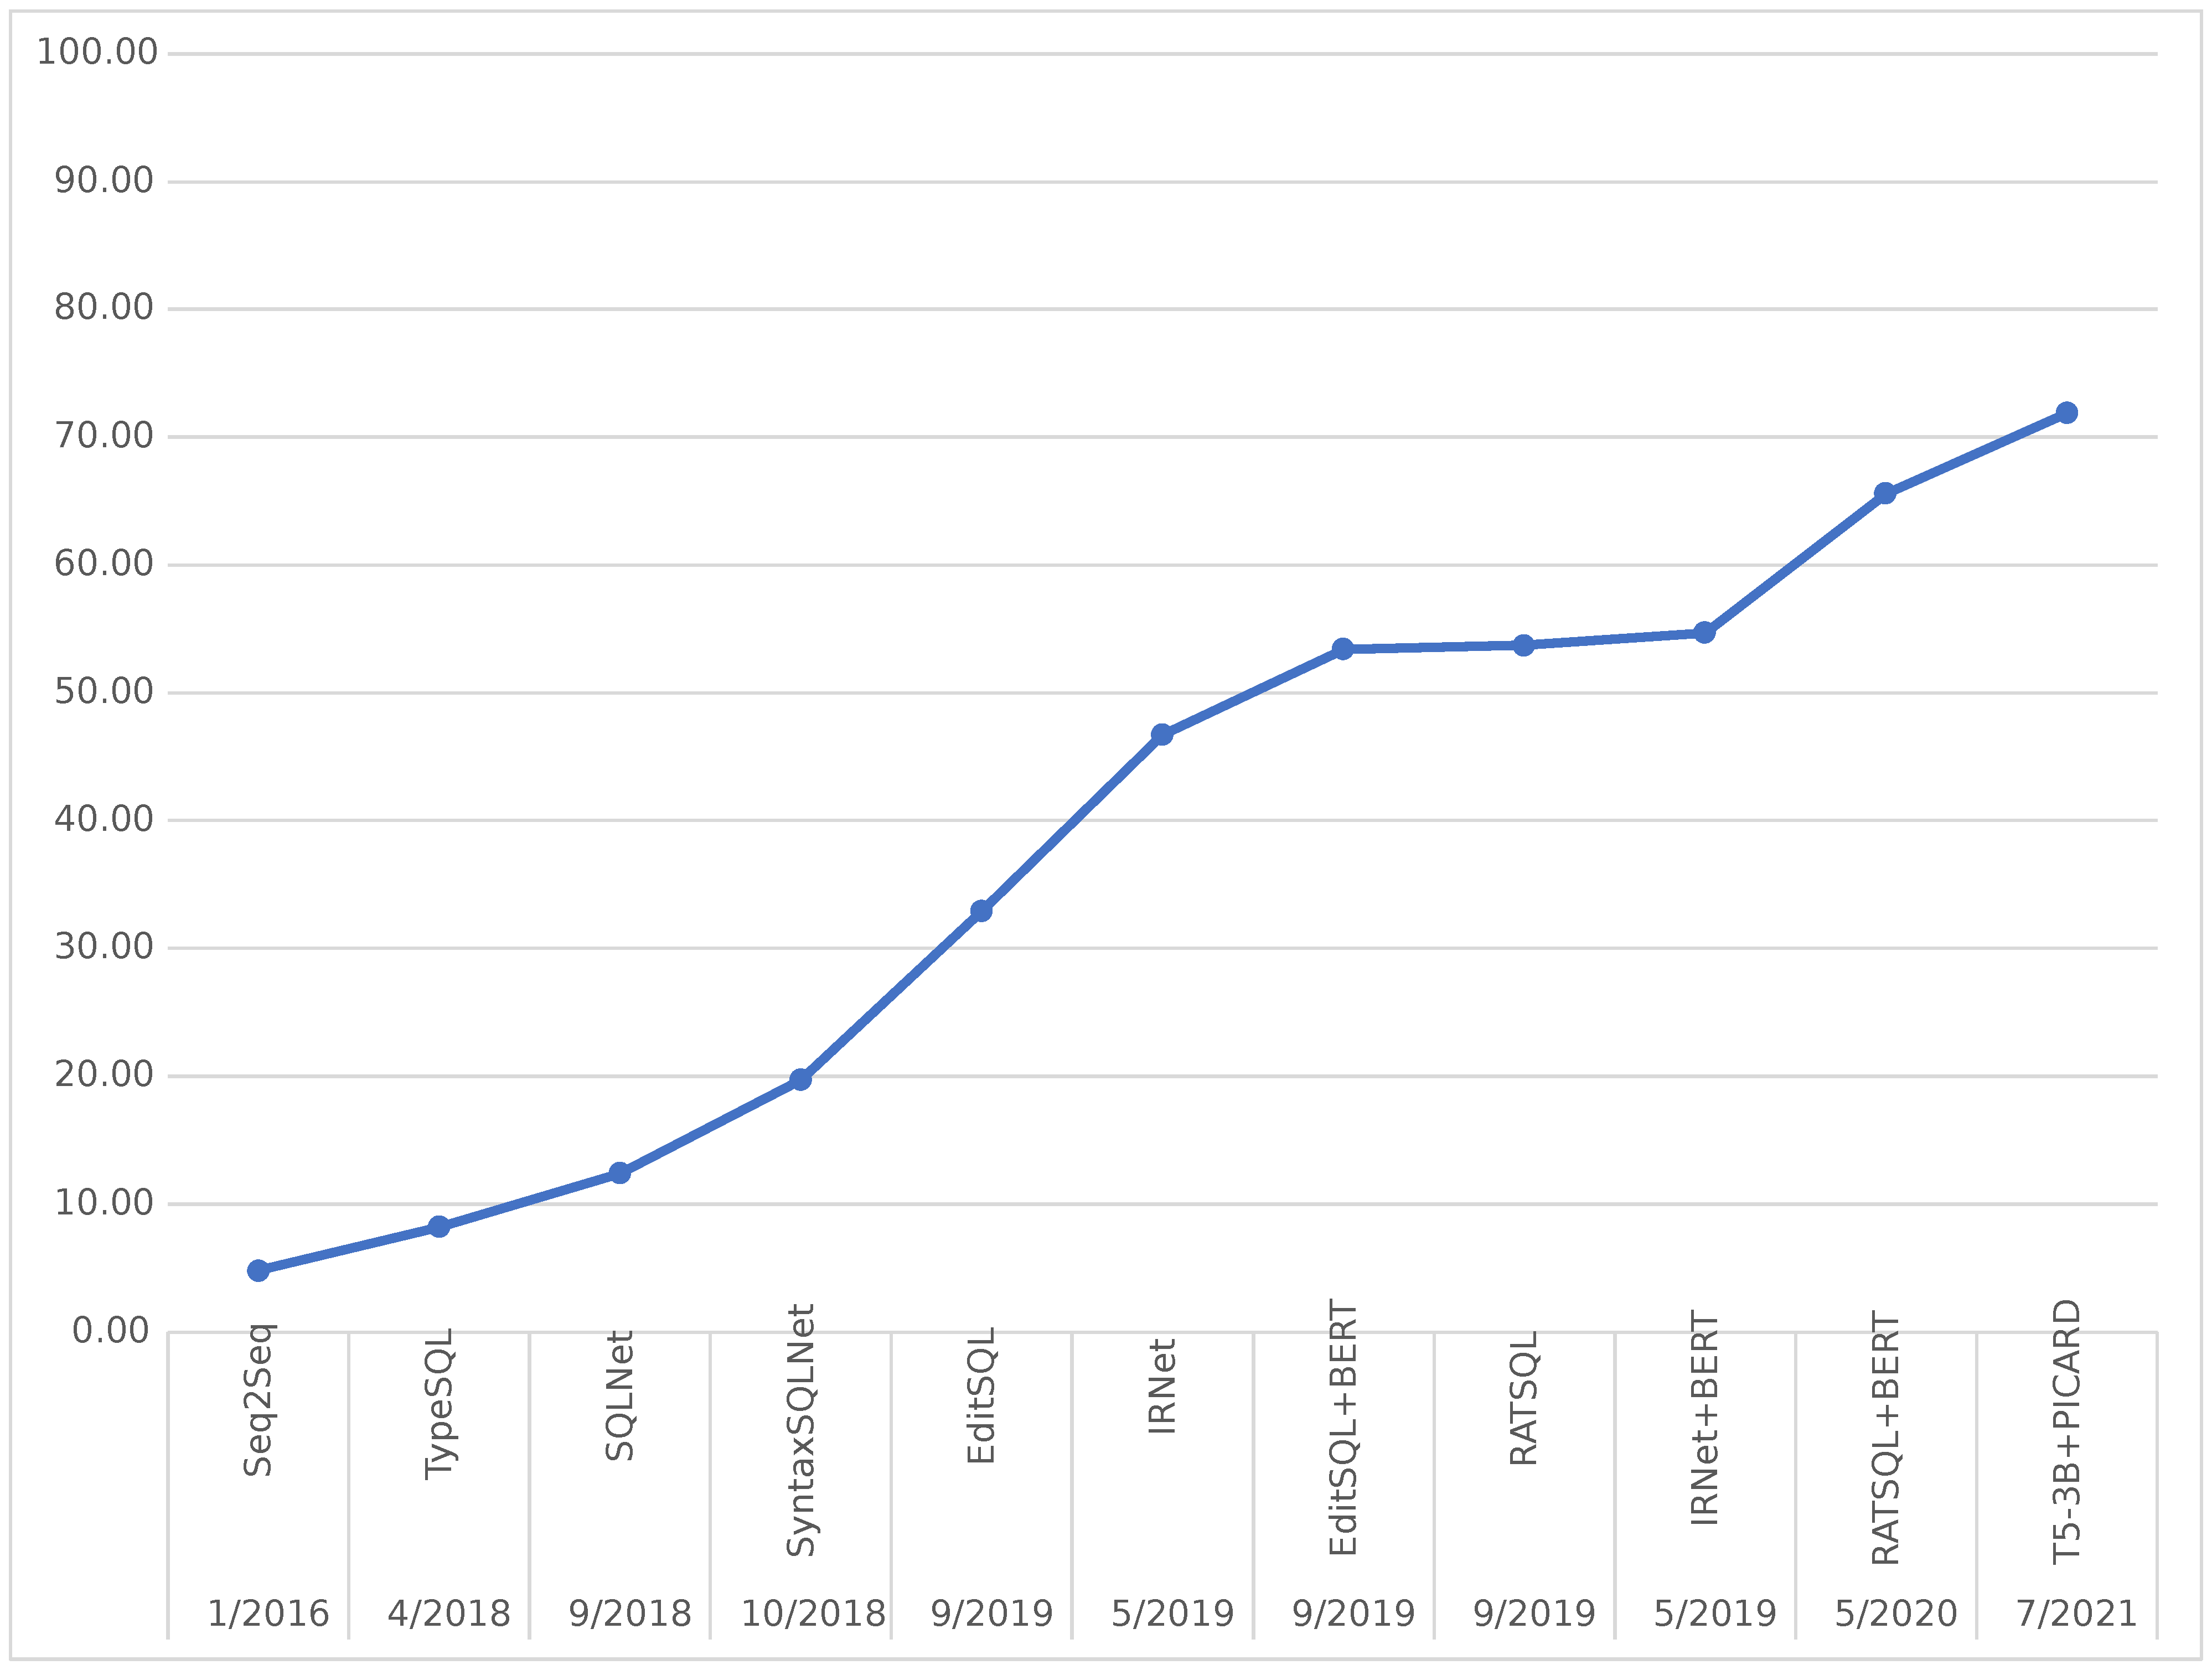
\includegraphics[width=0.99\linewidth]{pics/benchmarkeps}
    \caption{SPIDER benchmark Exact Match Results including our experiments}
    \label{fig:benchmark}
\end{figure}


Throughout this thesis, we have explored the advancements in Text-to-SQL models and their performance on the SPIDER benchmark. Our analysis revealed the significant progress made in the field, with more recent models demonstrating remarkable improvements in generating accurate SQL queries from natural language text.

The integration of powerful pre-trained language models, such as BERT, and cutting-edge architectures like T5 has played a vital role in the observed advancements. The models' ability to learn from limited labeled data, quickly adapt to new tasks or domains, and handle complex SQL queries has been substantially enhanced by employing techniques such as active learning, meta-learning, and multi-task learning.

In the following section, our experiments with ChatGPT-3.5 and ChatGPT-4.0 have showcased their superior performance, achieving scores of 81.30\% and 85.20\% on the SPIDER benchmark, respectively. These results highlight the potential of utilizing the latest huge language models for Text-to-SQL tasks, further pushing the boundaries of what is possible in this domain.

As the field of natural language processing continues to evolve, we can expect even more sophisticated models and techniques to emerge, enabling more accurate and efficient understanding and generation of SQL queries from natural language input. Future research in this area may focus on enhancing the models' ability to handle ambiguous or imprecise input, as well as exploring novel methods to improve their adaptability and generalization capabilities across diverse tasks and domains.

In the next section, we will illustrate different methods for evaluating the performance of such models.
\section{Evaluation Metrics} \label{eval}

Text-to-SQL tasks can be evaluated by multiple methods: Component Matching, Accurate matching rate and Execution accuracy rate. Predicted SQL statements are compared with standard statements to determine how accurate the match is.
By splitting the predicted SQL statement and definitive statement into multiple clauses according to keywords, we can solve the problem of matching errors caused by the order of the where clause. The matching is successful as long as the elements in both sets are the same.

% pics/acc1.png
\begin{figure}[htb]
    \centering
    \includegraphics[width=0.6\textwidth]{pics/acc1.png}
    % \caption{Accurate matching rate}
    \label{fig:acc1}
\end{figure}

When using the correct predicted SQL statements, the correct execution rate refers to the proportion of questions that can receive the correct answers from the database.

% pics/acc2.png
\begin{figure}[htb]
    \centering
    \includegraphics[width=0.4\textwidth]{pics/acc2.png}
    % \caption{Accuracy rate of the predicted SQL statements}
    \label{fig:acc2}
\end{figure}

% By predicting the key F1 values for SQL statements, the model can also be evaluated.

% % pics/f1.png
% \begin{figure}[htb]
%     \centering
%     \includegraphics[width=0.6\textwidth]{pics/f1.png}
%     % \caption{F1 score for SQL statements}
%     \label{fig:f1}
% \end{figure}

\subsection{Exact Matching}

Exact Matching\cite{xu_sqlnet_2017}, a popular metric for assessing the effectiveness of Text-to-SQL models, has drawbacks because it can yield erroneous negative results when the semantic parser can produce innovative syntactic structures. The predicted SQL query is compared against the corresponding reference SQL query. The model is considered to have produced the proper SQL query and is given a score of 1.0 if the predicted query is an exact duplicate of the reference query. The model is deemed to have generated an invalid query and obtains a score of 0.0 if the predicted query does not match the reference query. This metric aids in evaluating the overall syntactic and semantic accuracy of the generated query, but it ignores the query's constituent parts. This measure is a reliable evaluation technique because it verifies the entire SQL query. It is, therefore, a more stringent evaluation metric because it only deems a query correct if it exactly matches the reference question, down to the capitalization, spacing, and word order.


\subsection{Exact Set Matching}

Exact Set Matching compares the set of predicted SQL queries with the set of corresponding reference SQL queries, regardless of the elements' order, to assess the performance of a model. If every element from the set of predicted queries is included in the reference query, it returns a score of 1.0; otherwise, it returns a score of 0.0.

Generally, Exact Set Matching is more forgiving than Exact Matching, as the former does not take the order of elements or capitalization into account. On the other hand, Exact Matching is more stringent as it requires a perfect match including the order of words, capitalization and spaces, thus making it a reliable evaluation method.


\subsection{Component Matching}

Component matching\cite{yu_spider_2019} involves comparing the elements of the generated SQL query (e.g., the specified columns and tables) to the elements of the reference SQL query. Evaluation is based on the number of components that match correctly between the produced and reference queries, with a higher amount indicating improved performance. This metric assists in measuring the precision of the model's capability to create the correct SQL query components, but it does not factor in the full syntactic or semantic correctness of the query. Furthermore, it is utilized to assess the performance of various models on the same dataset.

\subsection{Execution Accuracy}

The execution accuracy metric\cite{yu_spider_2019} is a commonly used measure to evaluate the performance of text-to-SQL models. It determines the percentage of correctly generated SQL queries that can be successfully executed on the relevant database. In other words, it evaluates how well a model can convert text written in natural language into a SQL query that can successfully access the desired data from a database.

Execution accuracy is typically reported as a percentage, and higher values denote better performance. It is also important to remember that this metric only considers how correctly the generated SQL queries are syntactically and semantically and ignores how relevant or comprehensive the information is that is returned. Consequently, it is frequently combined with other metrics, such as informativeness, which assesses the accuracy and completeness of the retrieved data.

\section{Experiments}

Since SEOSS Dataset\cite{RATH2019104005} was only evaluated and trained with SQLNet and RatSQL in this section, we decided to investigate further by experimenting with this dataset using state-of-the-art solutions currently proposed for the SPIDER challenge. In order to determine the effectiveness of these methods, we compared the results obtained with those of SQLNet\ref{sec:sqlnet} and RatSQL\ref{sec:ratsql} from the SEOSS-Queries research paper\cite{TOMOVA2022108211}. The results of these experiments are presented in the following section, and they will demonstrate the potential of modern solutions for solving the SPIDER task.

\subsection{Limitations}

Our experiment requires a lot of computational resources as we mainly leverage the T5 model. We used a single Nvidia RTX 3070 16GB GPU with 40GB Memory for our experiment, which unfortunately limited us to smaller models with more restrictions. Despite these limitations, we were still able to achieve excellent results. If we had used a larger T5 model, such as T5-3B, we would have been able to reach much higher scores. Therefore, investing in a more powerful GPU for our experiment is something that we must consider in order to maximize our results.

\subsection{SEOSS + T5 PICARD Experiment}
After studying the SEOSS dataset, we decided to experiment with the PICARD model\ref{picard} to evaluate its performance against that of SQLNet and RatSQL. We decided to use the T5Base model for our experiment, as it is smaller than the T5-3B and T5-11B models used by most state-of-the-art studies. To ensure a fair comparison between the models, we used two beam sizes of 2 and 4 and the same evaluation metrics as SEOSS-SQLNet and SEOSS-RatSQL, which is "exact matching accuracy". We wanted to see if the PICARD model could achieve similar results to those of SQLNet and RatSQL, so we conducted our experiment with our findings. The results of our experiment are discussed in the following section and can be used to compare the performance of the PICARD model to the models used in the SEOSS study.
\footnote[1]{Link to the Github Page: \url{https://github.com/yazdipour/text-to-sql-seoss-t5}}

\begin{table}[!ht]
    \centering
    \begin{tabular}{|l|l|l|L|L|}
        \hline
        Model    & Picard Mode       & Beams & \textbf{Exact Matching Accuracy} & \textbf{Execution Accuracy} \\ \hline
        T5-base  & parse with guards & 2     & 0.3297                           & 0.3576                      \\ \hline
        T5-base  & lex               & 4     & 0.3071                           & 0.3039                      \\ \hline
        T5-base  & parse with guards & 4     & 0.3286                           & 0.3512                      \\ \hline
        T5-large & parse with guards & 4     & 0.4274                           & 0.4822                      \\ \hline
    \end{tabular}
    \caption{Expermiment Accuracy Results}
\end{table}

The table shows the results of various configurations of T5-base and T5-large models for natural language processing tasks. The configurations are differentiated by the Picard mode parse with guards or lex and the number of beams used in the beam search process 2 or 4.

Comparing the results, we can observe that:
\begin{itemize}
    \item The T5-large model generally performs better than the T5-base model in both exact matching accuracy and execution accuracy.
    \item The parse with guards Picard mode performs better than the lex Picard mode in both models.
    \item Using four beams instead of 2 in the beam search process improves the performance for both models and Picard modes.
    \item The highest exact matching accuracy is achieved by the T5-large model with parse with guards Picard mode and four beams 0.4274.
    \item The highest execution accuracy is also achieved by the T5-large model with parse with guards Picard mode and four beams 0.4822.
    \item Increasing beam size does not have a significant effect compared to changing the model and mode.
\end{itemize}


\begin{table}[h]
    \centering
    \begin{tabular}{|c|c|c|c|c|c|}
        \hline
        \multirow{2}*{Exact Match Accuracy} & easy  & medium & hard  & extra hard & all   \\
                                            & 392   & 378    & 77    & 84         & 931   \\ \hline
        SQLNet                              & 0.023 & 0.000  & 0.000 & 0.000      & 0.010 \\ \hline
        RatSQL + Glove                      & 0.309 & 0.214  & 0.091 & 0.000      & 0.224 \\ \hline
        RatSQL + Bert                       & 0.161 & 0.201  & 0.065 & 0.012      & 0.156 \\ \hline
        PICARD + T5Base + 4Beam             & 0.446 & 0.254  & 0.182 & 0.012      & 0.307 \\ \hline
        PICARD + T5Large + 4Beam            & 0.571 & 0.410  & 0.182 & 0.060      & 0.427 \\ \hline
    \end{tabular}
    \caption{Comparison between Exact Match Accuracy}
\end{table}

The table compares the exact match accuracy of various models that are not fine-tuned for our dataset. The models are evaluated on five difficulty levels: easy, medium, hard, extra hard, and all.

Comparing the results, we can observe that:
\begin{itemize}
    \item The PICARD + T5Large + 4Beam model has the highest exact match accuracy among all models and difficulty levels, with a maximum value of 0.571; this shows that this model is more generalized and can handle unseen databases quite well compared to other solutions.
    \item The PICARD + T5Base + 4Beam model performs better than the other models, with a maximum value of 0.446.
    \item The RatSQL models with Glove and Bert embeddings perform similarly, with a maximum value of 0.309 and 0.201, respectively.
    \item The SQLNet model performs the worst among all models, with a maximum value of 0.023.
    \item The extra hard and all difficulty levels generally have lower exact match accuracy values compared to the easy and medium levels. Amazingly T5 PICARD was still able to solve complex problems with a low percentage, yet better than the other models.
    \item Research in\cite{TOMOVA2022108211} shows that the trained RatSQL were able to achieve a high exact match accuracy. This is a good sign that the PICARD model can achieve high accuracy with a little fine-tuning.
\end{itemize}

\subsection{Recall and F1 Scores}

Here, we can observe the Recall and F1 scores of each SQL Keyword for the PICARD T5-Large 4-Beam experiment on the SEOSS dataset. We can see that PICARD has managed to attain a very impressive F1 score for the SEOSS dataset without even having to be specifically trained for our dataset. This is a very encouraging result and indicates that the model is able to generalize accurately across different domains. Moreover, it is essential to note that the F1 score obtained by the PICARD model was obtained without any additional fine-tuning. This is a testament to the robustness and capability of the model and further highlights its ability to generalize to different datasets.

We experimented with a variety of different parameters, including beam size, modes and model sizes, and spent multiple hours for each evaluation. These experiments have been carefully documented in the Appendix\ref{sec:appendix} of this thesis, where you can find the results in detail.


\begin{table}[h]
    \centering
    \begin{tabular}{|c|c|c|c|c|c|}
        \hline
        select           & 0.709 & 0.585 & 0.390 & 0.440 & 0.608 \\ \hline
        select(no AGG)   & 0.709 & 0.590 & 0.390 & 0.452 & 0.611 \\ \hline
        where            & 0.708 & 0.520 & 0.200 & 0.273 & 0.523 \\ \hline
        where(no OP)     & 0.750 & 0.526 & 0.200 & 0.325 & 0.548 \\ \hline
        group(no Having) & 0.429 & 0.754 & 0.914 & 0.286 & 0.691 \\ \hline
        group            & 0.000 & 0.726 & 0.914 & 0.214 & 0.649 \\ \hline
        order            & 0.000 & 0.143 & 0.543 & 0.310 & 0.343 \\ \hline
        and/or           & 0.987 & 0.997 & 1.000 & 0.983 & 0.992 \\ \hline
        keywords         & 0.823 & 0.725 & 0.649 & 0.417 & 0.704 \\ \hline
    \end{tabular}
    \caption{Partial Matching Recall - PICARD T5-Large 4-Beam}

\end{table}

\begin{table}[h]
    \centering
    \begin{tabular}{|c|c|c|c|c|c|}
        \hline
        select           & 0.743 & 0.625 & 0.395 & 0.490 & 0.644 \\ \hline
        select(no AGG)   & 0.743 & 0.631 & 0.395 & 0.503 & 0.647 \\ \hline
        where            & 0.723 & 0.593 & 0.230 & 0.323 & 0.576 \\ \hline
        where(no OP)     & 0.766 & 0.599 & 0.230 & 0.385 & 0.604 \\ \hline
        group(no Having) & 0.214 & 0.770 & 0.889 & 0.369 & 0.705 \\ \hline
        group            & 1.000 & 0.741 & 0.889 & 0.277 & 0.661 \\ \hline
        order            & 1.000 & 0.182 & 0.535 & 0.394 & 0.393 \\ \hline
        and/or           & 0.994 & 0.971 & 0.908 & 0.817 & 0.964 \\ \hline
        keywords         & 0.809 & 0.781 & 0.690 & 0.483 & 0.746 \\ \hline
    \end{tabular}
    \caption{Partial Matching F1 - PICARD T5-Large 4-Beam}
\end{table}
\subsection{EZ-PICARD}

% add image here
\begin{figure}[ht]
    \centering
    \includegraphics[width=1\textwidth]{pics/ez/ui.png}
    \caption{EZ-PICARD Web Application}
    \label{fig:ezpicard}
\end{figure}

\subsubsection{Microservices Practices}

% add image here
\begin{figure}[ht]
    \centering
    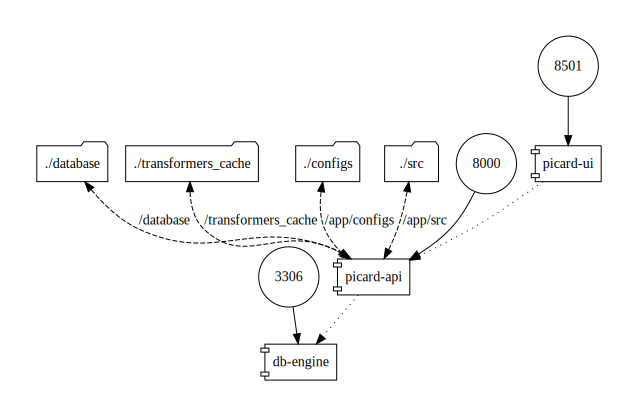
\includegraphics[width=0.8\textwidth]{pics/ez/map.png}
    \caption{EZ-PICARD Architecture}
\end{figure}


\subsubsection{DB Engines}

The Picard Method is a method for constrained inference on top of an existing model, but it is not a model itself. Currently, the PICARD parser and the supporting software are not supported for PostgreSQL, MySQL and others, which would require changes to the PICARD parser, translation of Spider databases and text-to-SQL data, and retraining models to produce MSSQL code. To use the Picard Method, a complex toolchain of Haskell code is built with CABAL and requires a complicated toolchain for the Facebook Thrift library.

After the setup, the Picard server can be started by running the compiled standalone executable PICARD. This executable is responsible for providing the necessary information to the user, such as specific parameters and options within the constrained inference. It is important to note that the Picard Method is not a full-fledged model; therefore, it is necessary to combine it with an existing model to get a complete inference system.

The thrift library is used for communication between the parser and the beam search algorithm. The parser, written in the efficient and powerful Haskell programming language, is used in combination with the hf transformers, which is a Python package. To further expand the scope of the system, new SQL engines can be supported by adding a parser for each one.

These parsers also need to be written in Haskell, as the existing SQLite parser is of limited use in this regard, as it has been written to work best on Spider's subset of SQLite and only supports part of the SQLite specification. This means that more advanced parsers must be created to maximize the system's capabilities. Additionally, these parsers need to be written with a high level of precision in order to ensure that the system can effectively communicate with various engines and databases.
\section{Conclusion}

\subsection{Future Work}

\subsection{Summary of findings}

\subsection{Limitations of the study}
\listoffigures
\addcontentsline{toc}{section}{List of Figures}

\listoftables
\addcontentsline{toc}{section}{List of Tables}

% -------------------- Bibliography --------------------
\renewcommand{\refname}{Bibliography}
\addcontentsline{toc}{section}{Bibliography}
\bibliographystyle{alpha}
\bibliography{bibs/litDB}

% -------------------- Appendix --------------------
% \clearpage
% \section{Appendix}
\label{sec:appendix}

\begin{itemize}
    \item T5 base
    \item Mode: Lex
    \item maximum tokens to check: 2
    \item number of beams: 2
\end{itemize}
% &easy                 &medium               &hard                 &extra                &all
% count                &392                  &378                  &77                   &84                   &931
% execution            &0.477                &0.251                &0.273                &0.000                &0.325
% exact match          &0.513                &0.291                &0.182                &0.000                &0.349
\begin{table}[h!]
    \centering
    \begin{tabular}{|c|c|c|c|c|c|}
        \hline
                         & easy  & medium & hard  & extra & all   \\ \hline
        select           & 0.873 & 0.624  & 0.469 & 0.500 & 0.717 \\ \hline
        select(no AGG)   & 0.873 & 0.642  & 0.469 & 0.500 & 0.724 \\ \hline
        where            & 0.882 & 0.824  & 0.308 & 0.421 & 0.780 \\ \hline
        where(no OP)     & 0.958 & 0.833  & 0.308 & 0.474 & 0.825 \\ \hline
        group(no Having) & 0.238 & 0.841  & 0.969 & 0.778 & 0.789 \\ \hline
        group            & 0.000 & 0.805  & 0.969 & 0.556 & 0.726 \\ \hline
        order            & 0.000 & 0.409  & 0.469 & 0.400 & 0.431 \\ \hline
        and/or           & 1.000 & 0.929  & 0.896 & 0.598 & 0.927 \\ \hline

        keywords         & 0.885 & 0.867  & 0.672 & 0.455 & 0.829 \\ \hline
    \end{tabular}
    \caption{PARTIAL MATCHING ACCURACY}
\end{table}

\begin{table}[h!]
    \centering
    \begin{tabular}{|c|c|c|c|c|c|}
        \hline
        select           & 0.597 & 0.373 & 0.390 & 0.131 & 0.447 \\ \hline
        select(no AGG)   & 0.597 & 0.384 & 0.390 & 0.131 & 0.451 \\ \hline
        where            & 0.756 & 0.429 & 0.229 & 0.104 & 0.477 \\ \hline
        where(no OP)     & 0.821 & 0.434 & 0.229 & 0.117 & 0.504 \\ \hline
        group(no Having) & 0.714 & 0.543 & 0.886 & 0.167 & 0.533 \\ \hline
        group            & 0.000 & 0.520 & 0.886 & 0.119 & 0.490 \\ \hline
        order            & 0.000 & 0.321 & 0.429 & 0.095 & 0.267 \\ \hline
        and/or           & 0.992 & 1.000 & 0.986 & 0.961 & 0.993 \\ \hline

        keywords         & 0.834 & 0.513 & 0.506 & 0.119 & 0.545 \\ \hline
    \end{tabular}
    \caption{PARTIAL MATCHING RECALL }

\end{table}
\begin{table}[h!]
    \centering
    \begin{tabular}{|c|c|c|c|c|c|}
        \hline
        select           & 0.709 & 0.467 & 0.426 & 0.208 & 0.551 \\ \hline
        select(no AGG)   & 0.709 & 0.480 & 0.426 & 0.208 & 0.556 \\ \hline
        where            & 0.814 & 0.564 & 0.262 & 0.167 & 0.592 \\ \hline
        where(no OP)     & 0.885 & 0.570 & 0.262 & 0.188 & 0.626 \\ \hline
        group(no Having) & 0.357 & 0.660 & 0.925 & 0.275 & 0.636 \\ \hline
        group            & 1.000 & 0.632 & 0.925 & 0.196 & 0.585 \\ \hline
        order            & 1.000 & 0.360 & 0.448 & 0.154 & 0.329 \\ \hline
        and/or           & 0.996 & 0.963 & 0.939 & 0.737 & 0.959 \\ \hline

        keywords         & 0.859 & 0.644 & 0.578 & 0.189 & 0.658 \\ \hline
    \end{tabular}
    \caption{PARTIAL MATCHING F1 }

\end{table}
\pagebreak
% easy                 medium               hard                 extra                all
% count                392                  378                  77                   84                   931

% execution            &0.477                &0.251                &0.273                &0.000                &0.325 \\ \hline
% \\ \hline
% exact match          &0.513                &0.291                &0.182                &0.000                &0.349 \\ \hline
% \\ \hline
\begin{itemize}
    \item T5 base
    \item Mode: parse with guards
    \item maximum tokens to check: 2
    \item number of beams: 2
\end{itemize}

\begin{table}[h!]
    \centering
    \begin{tabular}{|c|c|c|c|c|c|}
        \hline
        select           & 0.873 & 0.624 & 0.469 & 0.500 & 0.717 \\ \hline
        select(no AGG)   & 0.873 & 0.642 & 0.469 & 0.500 & 0.724 \\ \hline
        where            & 0.882 & 0.824 & 0.308 & 0.421 & 0.780 \\ \hline
        where(no OP)     & 0.958 & 0.833 & 0.308 & 0.474 & 0.825 \\ \hline
        group(no Having) & 0.238 & 0.841 & 0.969 & 0.778 & 0.789 \\ \hline
        group            & 0.000 & 0.805 & 0.969 & 0.556 & 0.726 \\ \hline
        order            & 0.000 & 0.409 & 0.469 & 0.400 & 0.431 \\ \hline
        and/or           & 1.000 & 0.929 & 0.896 & 0.598 & 0.927 \\ \hline

        keywords         & 0.885 & 0.867 & 0.672 & 0.455 & 0.829 \\ \hline
    \end{tabular}
    \caption{PARTIAL MATCHING ACCURACY}
\end{table}

\begin{table}[h!]
    \centering
    \begin{tabular}{|c|c|c|c|c|c|}
        \hline
        select           & 0.597 & 0.373 & 0.390 & 0.131 & 0.447 \\ \hline
        select(no AGG)   & 0.597 & 0.384 & 0.390 & 0.131 & 0.451 \\ \hline
        where            & 0.756 & 0.429 & 0.229 & 0.104 & 0.477 \\ \hline
        where(no OP)     & 0.821 & 0.434 & 0.229 & 0.117 & 0.504 \\ \hline
        group(no Having) & 0.714 & 0.543 & 0.886 & 0.167 & 0.533 \\ \hline
        group            & 0.000 & 0.520 & 0.886 & 0.119 & 0.490 \\ \hline
        order            & 0.000 & 0.321 & 0.429 & 0.095 & 0.267 \\ \hline
        and/or           & 0.992 & 1.000 & 0.986 & 0.961 & 0.993 \\ \hline

        keywords         & 0.834 & 0.513 & 0.506 & 0.119 & 0.545 \\ \hline
    \end{tabular}
    \caption{PARTIAL MATCHING RECALL }

\end{table}
\begin{table}[h!]
    \centering
    \begin{tabular}{|c|c|c|c|c|c|}
        \hline
        select           & 0.709 & 0.467 & 0.426 & 0.208 & 0.551 \\ \hline
        select(no AGG)   & 0.709 & 0.480 & 0.426 & 0.208 & 0.556 \\ \hline
        where            & 0.814 & 0.564 & 0.262 & 0.167 & 0.592 \\ \hline
        where(no OP)     & 0.885 & 0.570 & 0.262 & 0.188 & 0.626 \\ \hline
        group(no Having) & 0.357 & 0.660 & 0.925 & 0.275 & 0.636 \\ \hline
        group            & 1.000 & 0.632 & 0.925 & 0.196 & 0.585 \\ \hline
        order            & 1.000 & 0.360 & 0.448 & 0.154 & 0.329 \\ \hline
        and/or           & 0.996 & 0.963 & 0.939 & 0.737 & 0.959 \\ \hline

        keywords         & 0.859 & 0.644 & 0.578 & 0.189 & 0.658 \\ \hline
    \end{tabular}
    \caption{PARTIAL MATCHING F1 }

\end{table}
\pagebreak
\begin{itemize}
    \item T5 base
    \item Mode: Lex
    \item maximum tokens to check: 2
    \item number of beams: 4
\end{itemize}

% easy                 medium               hard                 extra                all
% count                392                  378                  77                   84                   931

% execution            &0.401                &0.212                &0.273                &0.012                &0.278


% exact match          &0.446                &0.254                &0.182                &0.012                &0.307

\begin{table}[h!]
    \centering
    \begin{tabular}{|c|c|c|c|c|c|}
        \hline
        select           & 0.858 & 0.623 & 0.483 & 0.571 & 0.713 \\ \hline
        select(no AGG)   & 0.858 & 0.643 & 0.483 & 0.571 & 0.721 \\ \hline
        where            & 0.863 & 0.804 & 0.333 & 0.474 & 0.771 \\ \hline
        where(no OP)     & 0.950 & 0.814 & 0.333 & 0.526 & 0.820 \\ \hline
        group(no Having) & 0.192 & 0.842 & 0.968 & 0.750 & 0.759 \\ \hline
        group            & 0.000 & 0.812 & 0.968 & 0.500 & 0.699 \\ \hline
        order            & 0.000 & 0.391 & 0.484 & 0.444 & 0.431 \\ \hline
        and/or           & 1.000 & 0.921 & 0.870 & 0.602 & 0.921 \\ \hline

        keywords         & 0.836 & 0.833 & 0.673 & 0.476 & 0.797 \\ \hline
    \end{tabular}
    \caption{PARTIAL MATCHING ACCURACY}

\end{table}
\begin{table}[h!]
    \centering
    \begin{tabular}{|c|c|c|c|c|c|}
        \hline
        select           & 0.538 & 0.341 & 0.377 & 0.143 & 0.409 \\ \hline
        select(no AGG)   & 0.538 & 0.352 & 0.377 & 0.143 & 0.414 \\ \hline
        where            & 0.714 & 0.418 & 0.229 & 0.117 & 0.460 \\ \hline
        where(no OP)     & 0.786 & 0.423 & 0.229 & 0.130 & 0.489 \\ \hline
        group(no Having) & 0.714 & 0.486 & 0.857 & 0.143 & 0.486 \\ \hline
        group            & 0.000 & 0.469 & 0.857 & 0.095 & 0.448 \\ \hline
        order            & 0.000 & 0.321 & 0.429 & 0.095 & 0.267 \\ \hline
        and/or           & 0.995 & 1.000 & 0.971 & 0.980 & 0.994 \\ \hline

        keywords         & 0.789 & 0.462 & 0.481 & 0.119 & 0.505 \\ \hline
    \end{tabular}
    \caption{PARTIAL MATCHING RECALL }

\end{table}

\begin{table}[h!]
    \centering
    \begin{tabular}{|c|c|c|c|c|c|}
        \hline
        select           & 0.661 & 0.441 & 0.423 & 0.229 & 0.520 \\ \hline
        select(no AGG)   & 0.661 & 0.455 & 0.423 & 0.229 & 0.526 \\ \hline
        where            & 0.782 & 0.550 & 0.271 & 0.188 & 0.576 \\ \hline
        where(no OP)     & 0.860 & 0.557 & 0.271 & 0.208 & 0.613 \\ \hline
        group(no Having) & 0.303 & 0.616 & 0.909 & 0.240 & 0.593 \\ \hline
        group            & 1.000 & 0.594 & 0.909 & 0.160 & 0.546 \\ \hline
        order            & 1.000 & 0.353 & 0.455 & 0.157 & 0.329 \\ \hline
        and/or           & 0.997 & 0.959 & 0.918 & 0.746 & 0.956 \\ \hline

        keywords         & 0.812 & 0.595 & 0.561 & 0.190 & 0.618 \\ \hline
    \end{tabular}
    \caption{PARTIAL MATCHING F1 }

\end{table}
\pagebreak
\begin{itemize}
    \item T5 base
    \item Mode: parse with guards
    \item maximum tokens to check: 2
    \item number of beams: 4
\end{itemize}

% easy                 medium               hard                 extra                all
% count                392                  378                  77                   84                   931

% execution            &0.426                &0.272                &0.273                &0.024                &0.315


% exact match          &0.467                &0.283                &0.182                &0.024                &0.329

\begin{table}[h!]
    \centering
    \begin{tabular}{|c|c|c|c|c|c|}
        \hline
        select           & 0.757 & 0.537 & 0.417 & 0.469 & 0.618 \\ \hline
        select(no AGG)   & 0.757 & 0.559 & 0.417 & 0.469 & 0.627 \\ \hline
        where            & 0.779 & 0.746 & 0.250 & 0.433 & 0.695 \\ \hline
        where(no OP)     & 0.812 & 0.811 & 0.250 & 0.467 & 0.738 \\ \hline
        group(no Having) & 0.044 & 0.678 & 0.971 & 0.478 & 0.588 \\ \hline
        group            & 0.000 & 0.658 & 0.971 & 0.391 & 0.561 \\ \hline
        order            & 0.000 & 0.269 & 0.457 & 0.526 & 0.407 \\ \hline
        and/or           & 1.000 & 0.910 & 0.883 & 0.619 & 0.919 \\ \hline

        keywords         & 0.742 & 0.785 & 0.667 & 0.422 & 0.729 \\ \hline
    \end{tabular}
    \caption{PARTIAL MATCHING ACCURACY}

\end{table}
\begin{table}[h!]
    \centering
    \begin{tabular}{|c|c|c|c|c|c|}
        \hline
        select           & 0.653 & 0.442 & 0.390 & 0.274 & 0.511 \\ \hline
        select(no AGG)   & 0.653 & 0.460 & 0.390 & 0.274 & 0.519 \\ \hline
        where            & 0.690 & 0.464 & 0.171 & 0.169 & 0.475 \\ \hline
        where(no OP)     & 0.720 & 0.505 & 0.171 & 0.182 & 0.504 \\ \hline
        group(no Having) & 0.286 & 0.589 & 0.971 & 0.262 & 0.579 \\ \hline
        group            & 0.000 & 0.571 & 0.971 & 0.214 & 0.552 \\ \hline
        order            & 0.000 & 0.250 & 0.457 & 0.238 & 0.314 \\ \hline
        and/or           & 0.992 & 0.997 & 1.000 & 1.000 & 0.995 \\ \hline

        keywords         & 0.823 & 0.605 & 0.571 & 0.226 & 0.610 \\ \hline
    \end{tabular}
    \caption{PARTIAL MATCHING RECALL }

\end{table}
\begin{table}[h!]
    \centering
    \begin{tabular}{|c|c|c|c|c|c|}
        \hline
        select           & 0.701 & 0.485 & 0.403 & 0.346 & 0.560 \\ \hline
        select(no AGG)   & 0.701 & 0.505 & 0.403 & 0.346 & 0.568 \\ \hline
        where            & 0.732 & 0.572 & 0.203 & 0.243 & 0.564 \\ \hline
        where(no OP)     & 0.763 & 0.623 & 0.203 & 0.262 & 0.599 \\ \hline
        group(no Having) & 0.077 & 0.630 & 0.971 & 0.338 & 0.584 \\ \hline
        group            & 1.000 & 0.612 & 0.971 & 0.277 & 0.556 \\ \hline
        order            & 1.000 & 0.259 & 0.457 & 0.328 & 0.355 \\ \hline
        and/or           & 0.996 & 0.951 & 0.938 & 0.765 & 0.956 \\ \hline

        keywords         & 0.780 & 0.684 & 0.615 & 0.295 & 0.665 \\ \hline
    \end{tabular}
    \caption{PARTIAL MATCHING F1 }

\end{table}
\pagebreak
\begin{itemize}
    \item T5 large
    \item Mode: parse with guards
    \item maximum tokens to check: 2
    \item number of beams: 4
\end{itemize}

% easy                 medium               hard                 extra                all
% count                392                  378                  77                   84                   931
% execution            &0.531                &0.399                &0.299                &0.060                &0.416
% exact match          &0.571                &0.410                &0.182                &0.060                &0.427

\begin{table}[h!]
    \centering
    \begin{tabular}{|c|c|c|c|c|c|}
        \hline
        select           & 0.781 & 0.672 & 0.400 & 0.552 & 0.684 \\ \hline
        select(no AGG)   & 0.781 & 0.678 & 0.400 & 0.567 & 0.688 \\ \hline
        where            & 0.739 & 0.689 & 0.269 & 0.396 & 0.642 \\ \hline
        where(no OP)     & 0.783 & 0.696 & 0.269 & 0.472 & 0.673 \\ \hline
        group(no Having) & 0.143 & 0.786 & 0.865 & 0.522 & 0.719 \\ \hline
        group            & 0.000 & 0.756 & 0.865 & 0.391 & 0.675 \\ \hline
        order            & 0.000 & 0.250 & 0.528 & 0.542 & 0.462 \\ \hline
        and/or           & 1.000 & 0.947 & 0.831 & 0.699 & 0.937 \\ \hline

        keywords         & 0.796 & 0.846 & 0.735 & 0.574 & 0.792 \\ \hline
    \end{tabular}
    \caption{PARTIAL MATCHING ACCURACY}

\end{table}

\begin{table}[h!]
    \centering
    \begin{tabular}{|c|c|c|c|c|c|}
        \hline
        select           & 0.709 & 0.585 & 0.390 & 0.440 & 0.608 \\ \hline
        select(no AGG)   & 0.709 & 0.590 & 0.390 & 0.452 & 0.611 \\ \hline
        where            & 0.708 & 0.520 & 0.200 & 0.273 & 0.523 \\ \hline
        where(no OP)     & 0.750 & 0.526 & 0.200 & 0.325 & 0.548 \\ \hline
        group(no Having) & 0.429 & 0.754 & 0.914 & 0.286 & 0.691 \\ \hline
        group            & 0.000 & 0.726 & 0.914 & 0.214 & 0.649 \\ \hline
        order            & 0.000 & 0.143 & 0.543 & 0.310 & 0.343 \\ \hline
        and/or           & 0.987 & 0.997 & 1.000 & 0.983 & 0.992 \\ \hline

        keywords         & 0.823 & 0.725 & 0.649 & 0.417 & 0.704 \\ \hline
    \end{tabular}
    \caption{PARTIAL MATCHING RECALL }

\end{table}

\begin{table}[h!]
    \centering
    \begin{tabular}{|c|c|c|c|c|c|}
        \hline
        select           & 0.743 & 0.625 & 0.395 & 0.490 & 0.644 \\ \hline
        select(no AGG)   & 0.743 & 0.631 & 0.395 & 0.503 & 0.647 \\ \hline
        where            & 0.723 & 0.593 & 0.230 & 0.323 & 0.576 \\ \hline
        where(no OP)     & 0.766 & 0.599 & 0.230 & 0.385 & 0.604 \\ \hline
        group(no Having) & 0.214 & 0.770 & 0.889 & 0.369 & 0.705 \\ \hline
        group            & 1.000 & 0.741 & 0.889 & 0.277 & 0.661 \\ \hline
        order            & 1.000 & 0.182 & 0.535 & 0.394 & 0.393 \\ \hline
        and/or           & 0.994 & 0.971 & 0.908 & 0.817 & 0.964 \\ \hline

        keywords         & 0.809 & 0.781 & 0.690 & 0.483 & 0.746 \\ \hline
    \end{tabular}
    \caption{PARTIAL MATCHING F1 }
\end{table}
% \addcontentsline{toc}{section}{Appendix} % Add the appendix to the table of contents manually

\end{document}